% ---------------------------------------------------------------------------
% Author guideline and sample document for EG publication using LaTeX2e input
% D.Fellner, v1.15, Dec 14, 2018

\documentclass{egpubl}
\usepackage{eurovis2022}

% --- for  Annual CONFERENCE
% \ConferenceSubmission   % uncomment for Conference submission
% \ConferencePaper        % uncomment for (final) Conference Paper
% \STAR                   % uncomment for STAR contribution
% \Tutorial               % uncomment for Tutorial contribution
% \ShortPresentation      % uncomment for (final) Short Conference Presentation
% \Areas                  % uncomment for Areas contribution
% \MedicalPrize           % uncomment for Medical Prize contribution
% \Education              % uncomment for Education contribution
% \Poster                 % uncomment for Poster contribution
% \DC                     % uncomment for Doctoral Consortium
%
% --- for  CGF Journal
% \JournalSubmission    % uncomment for submission to Computer Graphics Forum
% \JournalPaper         % uncomment for final version of Journal Paper
%
% --- for  CGF Journal: special issue
% \SpecialIssueSubmission    % uncomment for submission to , special issue
\SpecialIssuePaper         % uncomment for final version of Computer Graphics Forum, special issue
%                          % EuroVis, SGP, Rendering, PG
% --- for  EG Workshop Proceedings
% \WsSubmission      % uncomment for submission to EG Workshop
% \WsPaper           % uncomment for final version of EG Workshop contribution
% \WsSubmissionJoint % for joint events, for example ICAT-EGVE
% \WsPaperJoint      % for joint events, for example ICAT-EGVE
% \Expressive        % for SBIM, CAe, NPAR
% \DigitalHeritagePaper
% \PaperL2P          % for events EG only asks for License to Publish

% --- for EuroVis 
% for full papers use \SpecialIssuePaper
% \STAREurovis   % for EuroVis additional material 
% \EuroVisPoster % for EuroVis additional material 
% \EuroVisShort  % for EuroVis additional material

% !! *please* don't change anything above
% !! unless you REALLY know what you are doing
% ------------------------------------------------------------------------
\usepackage[T1]{fontenc}
\usepackage{dfadobe}  

\usepackage{cite}  % comment out for biblatex with backend=biber
% \usepackage{tabu}
% ---------------------------
%\biberVersion
\BibtexOrBiblatex
%\usepackage[backend=biber,bibstyle=EG,citestyle=alphabetic,backref=true]{biblatex} 
%\addbibresource{chartability.bib}
% ---------------------------  
\electronicVersion
\PrintedOrElectronic
% for including postscript figures
% mind: package option 'draft' will replace PS figure by a filename within a frame
\ifpdf \usepackage[pdftex]{graphicx} \pdfcompresslevel=9
\else \usepackage[dvips]{graphicx} \fi

\usepackage{egweblnk}
% \usepackage{url}
\def\UrlBreaks{\do\/\do-}
% \usepackage{breakurl}
% \usepackage[breaklinks]{hyperref}
\usepackage{booktabs}

\usepackage{xspace,xpunctuate}
\newcommand{\ie}{{i.e.,}\xspace}
\newcommand{\eg}{{e.g.,}\xspace}
\newcommand{\ea}{{et~al\xperiod}\xspace}
\newcommand{\aka}{{a.k.a.}\xspace}
\newcommand{\etc}{{etc\xperiod}\xspace}
% \setlength\extrarowheight{0.16cm}
% \renewcommand{\arraystretch}{15}

% end of prologue

% \input{EGauthorGuidelines-body.inc}


% ---------------------------------------------------------------------
% EG author guidelines plus sample file for EG publication using LaTeX2e input
% D.Fellner, v2.03, Dec 14, 2018


\title[Chartability]%
      {How accessible is my visualization? Evaluating visualization accessibility with Chartability}

% for anonymous conference submission please enter your SUBMISSION ID
% instead of the author's name (and leave the affiliation blank) !!
% for final version: please provide your *own* ORCID in the brackets following \orcid; see https://orcid.org/ for more details.
% \author[Submission 1160]{Submission ID 1160}

\author[F. Elavsky, C. Bennett, \& D. Moritz]
{\parbox{\textwidth}{\centering Frank Elavsky,$^{1}$\orcid{0000-0002-6849-5893}
        Cynthia Bennett,$^{1}$
        and Dominik Moritz$^{1}$\orcid{0000-0002-3110-1053}
%        S. Spencer$^2$\thanks{Chairman Siggraph Publications Board}  
        }
        \\
% For Computer Graphics Forum: Please use the abbreviation of your first name.
{\parbox{\textwidth}{\centering $^1$Carnegie Mellon University, Human-Computer Interaction Institute\\
%        $^2$ Another Department to illustrate the use in papers from authors
%             with different affiliations
       } 
}
}
% ------------------------------------------------------------------------

% if the Editors-in-Chief have given you the data, you may uncomment
% the following five lines and insert it here
%
% \volume{36}   % the volume in which the issue will be published;
% \issue{1}     % the issue number of the publication
% \pStartPage{1}      % set starting page


%-------------------------------------------------------------------------
\begin{document}

\def\arraystretch{1.3}

% \teaser{
%  \includegraphics[width=\linewidth]{eg_new}
%  \centering
%   \caption{New EG Logo}
% \label{fig:teaser}
% }

\maketitle
%-------------------------------------------------------------------------
\begin{abstract}
Novices and experts have struggled to evaluate the accessibility of data visualizations because there are no common shared guidelines across environments, platforms, and contexts in which data visualizations are authored. Between non-specific standards bodies like WCAG, emerging research, and guidelines from specific communities of practice, it is hard to organize knowledge on how to evaluate accessible data visualizations. We present Chartability, a set of heuristics synthesized from these various sources which enables designers, developers, researchers, and auditors to evaluate data-driven visualizations and interfaces for visual, motor, vestibular, neurological, and cognitive accessibility. In this paper, we outline our process of making a set of heuristics and accessibility principles for Chartability and highlight key features in the auditing process. Working with participants on real projects, we found that data practitioners with a novice level of accessibility skills were more confident and found auditing to be easier after using Chartability. Expert accessibility practitioners were eager to integrate Chartability into their own work. Reflecting on Chartability’s development and the preliminary user evaluation, we discuss tradeoffs of open projects, working with high-risk evaluations like auditing projects in the wild, and challenge future research projects at the intersection of visualization and accessibility to consider the broad intersections of disabilities.

%-------------------------------------------------------------------------
%  ACM CCS 1998
%  (see https://www.acm.org/publications/computing-classification-system/1998)
% \begin{classification} % according to https://www.acm.org/publications/computing-classification-system/1998
% \CCScat{Computer Graphics}{I.3.3}{Picture/Image Generation}{Line and curve generation}
% \end{classification}
%-------------------------------------------------------------------------
%  ACM CCS 2012
%   (see https://www.acm.org/publications/class-2012)
%The tool at \url{http://dl.acm.org/ccs.cfm} can be used to generate
% CCS codes.
%Example:
\begin{CCSXML}
<ccs2012>
<concept>
<concept_id>10003120.10003145.10011770</concept_id>
<concept_desc>Human-centered computing~Visualization design and evaluation methods</concept_desc>
<concept_significance>500</concept_significance>
</concept>
<concept>
<concept_id>10003120.10011738.10011774</concept_id>
<concept_desc>Human-centered computing~Accessibility design and evaluation methods</concept_desc>
<concept_significance>500</concept_significance>
</concept>
<concept>
<concept_id>10003120.10003121.10003122.10010855</concept_id>
<concept_desc>Human-centered computing~Heuristic evaluations</concept_desc>
<concept_significance>500</concept_significance>
</concept>
</ccs2012>
\end{CCSXML}

\ccsdesc[500]{Human-centered computing~Visualization design and evaluation methods}
\ccsdesc[500]{Human-centered computing~Accessibility design and evaluation methods}
\ccsdesc[500]{Human-centered computing~Heuristic evaluations}


\printccsdesc   
\end{abstract}
%-------------------------------------------------------------------------
\section{Introduction}

26\% of people in the United States self-report living with at least one disability~\cite{cdc_disability_2018}. Of those, 13.7\% live with a mobility disability and 10.8\% with a cognitive disability. Globally, the World Health Organization reports that 29\% of the world lives with uncorrected or uncorrectable blindness, low vision, or moderate to severe visual impairment~\cite{noauthor_world_nodate}. Access is a significant inclusion effort that has broad international impact, especially for data visualization. 

Accessibility is the practice of making information, content, and functionality fully available to and usable by people with disabilities. As part of this process, practitioners need to be able to identify accessibility barriers. While general accessibility standards help, evaluating the inaccessibility of complex data systems can be a daunting and often expensive task. State-of-the art automated compliance checkers only find 57\% of accessibility errors~\cite{noauthor_study_2021}, meaning accessible experiences must still be manually designed and checked for quality. And following standards may only account for up to half of the needs of people with disabilities \cite{power_2012} anyway. Additionally, the intended wide applicability of these general standards means they fall short for information-rich systems, such as data visualizations (which use size, color, angles, shapes, and other dimensions to encode information). These specific contexts, communities, and libraries that deal with data visualizations and information-rich interfaces often have their own tools and guidelines for use, but they seldom include accessibility. Finally, research at the intersection of data visualization and accessibility has yet to meaningfully permeate data visualization tools and communities and primarily focuses on blindness and low vision, neglecting diverse accessibility needs of people with other disabilities.  

Synthesizing evolving accessibility standards, research findings, and artifacts from communities of practice into usable knowledge for a specific, evolving domain is a wicked problem. To address this, we present Chartability. Chartability is an accessibility evaluation system specific to data visualizations and interfaces which aims to help practitioners answer the question, ``how accessible is my data visualization?'' Chartability organizes knowledge from disparate bodies of work into testable heuristics based on the functional accessibility principles POUR (Perceivable, Operable, Understandable, and Robust)~\cite{initiative_wai_accessibility_nodate} and 3 novel principles CAF (Compromising, Assistive, and Flexible), which we added to attend to the unique qualities and demands of data visualizations. We refer to these 7 heuristic principles as POUR+CAF. Chartability is a community-contributed project that leverages the governance strategies of open source projects as a way to address the complex dual-evolution of both accessibility and data interaction practices. 

We additionally present an initial, light evaluation of Chartability from the experience of practitioners using it. We set out to see if using Chartability reduces the barrier of entry into this work for accessibility novices and if accessibility experts had any feedback to share about its use. We gave practitioners introductory material for Chartability and instructed them to use it according to their needs. We found that before using Chartability only accessibility experts believed auditing data visualizations to be somewhat easy or easy, while the other group believed auditing data visualizations to be somewhat hard or hard. All novice accessibility practitioners became more confident after using Chartability and believed auditing data visualizations for accessibility to be less difficult. Conversely while the expert accessibility practitioners were already confident in their ability to evaluate accessibility (and all unanimously had no change in their before and after evaluations), they were excited to adopt Chartability into their set of auditing resources. 

Our work sets out to acknowledge that data practitioners face significant barriers when first making data visualizations, systems, and experiences accessible. While Chartability contributes to filling gaps and organizing knowledge, it also challenges visualization and data interaction researchers to explore new horizons of possibilities in this space. As such, we conclude with recommendations for future research at the crossroads of data visualization and accessibility. 

\section{Existing Work in Data Visualization and Accessibility}

While recent works at the intersection of data visualization and accessibility are promising, they do not provide a consistent and unified methodology for designers to evaluate the accessibility of their work across the broad spectrum of disability considerations.

\subsection{Research Advancements in Data Visualization and Accessibility}
In parallel to Mack \ea's ``What do we mean by Accessibility Research?''~\cite{mack_what_2021} when we asked ``What do we mean by data visualization accessibility research?'' we found that nearly all topics of study were vision-related. Largely, access issues other than vision that affect data visualization (such as cognitive/neurological, vestibular, and motor concerns) are almost entirely unserved in this research space. Kim \ea found that 56 papers have been published between 1999 and 2020 that focus on vision-related accessibility (not including color vision deficiency), with only 3 being published at a visualization venue (and only recently since 2018)~\cite{kim_accessible_2021}. Marriott \ea found that there is no research at all that engages motor accessibility~\cite{marriott_inclusive_2021}. We have found 2 papers that engage cognitive/neurological disability in visualization and 1 student poster from IEEE Vis, which are all recent (specifically intellectual developmental disabilities~\cite{wu_understanding_2021} and seizure risk~\cite{south_generating_2020,south_detecting_2021}). We found no papers that engage vestibular accessibility, such as motion and animation-related accessibility. We also found that there is no research specific to low vision disabilities (not blindness or color vision deficiency) unless conflated with screen reader usage in data visualization. Blind and low vision people are often researched together, but in practice may use different assistive technologies (such as magnifiers and contrast enhancers) and have different interaction practices (such as a combination of sight, magnification, and screen reader use)~\cite{szpiro_2016}. 

Since the 1990s, the most prominent and active accessibility topic in visualization has been color vision deficiency~\cite{chaparro_applications_2017,nunez_optimizing_2018,oliveira_towards_2013,9023497,martinez_methodology_2021}. Research projects that explore tactile sensory substitutions have been a topic in computational sciences dating back to the 1983~\cite{geldard_tactual_1983}, with tactile sensory substitutions being used for maps and charts as far back as the 1830s~\cite{noauthor_extensive_2016}. Sonification used both in comparison to and alongside visualization and tactile methods for accessibility dates as far back as 1985~\cite{mansur_sound_1985,flowers_cross-modal_1997,brewster_visualization_2002,mcgookin_soundbar_2006,zhao_data_2008,cullen_co-designing_2019}. Some more recent work has explored robust screen reader data interaction techniques~\cite{miesenberger_accessible_2018,sorge_polyfilling_2016}, screen reader user experiences with digital, 2-D spatial representations, including data visualizations~\cite{schaadhardt_understanding_2021,sharif_understanding_2021}, dug deeper into the semantic layers of effective chart descriptions~\cite{lundgard_accessible_22}, and investigated how to better understand the role of sensory substitution~\cite{chundury_towards_2022}. Jung \ea offer guidance that expands beyond commonly cited literature that chart descriptions are preferably between 2 and 8 sentences long, written in plain language, and with consideration for the order of information and navigation~\cite{jung_communicating_2022}. We find all of this emerging work promising and foundational.

Despite this promising work emerging, we also want to acknowledge a spectrum of other work that exists at the intersection of accessibility and data visualization that does not serve the goals of our project. There is significant research that explores automatic or extracted textual descriptions~\cite{choi_visualizing_2019,balaji_chart-text_2018,chen_neural_2019,chen_figure_2020,lai_automatic_2020,obeid_chart--text_2020,qian_generating_2021,sharif_evographs_2018} and haptic graphs and tactile interfaces~\cite{aldrich_talk_2008,bornschein_collaborative_2015, brown_viztouch_2012,butler_technology_2021,gallace_what_2011,geldard_tactual_1983,jansen_opportunities_2015,jayant_automated_2007,lederman_perception_1986,schneider_constructing_nodate,shi_tickers_2016,baker_2016}. These research projects produce artifacts that are high-cost for individual use, some are not robust enough to interpret complex visualizations effectively, and several have not included people with disabilities. Since our goal is to synthesize knowledge for practitioner accessibility work, we also acknowledge that some of these projects did not follow standards during their research project and in their output, such as using Web Content Accessibility Guidelines~\cite{noauthor_web_nodate} or The American Printing House for the Blind and Braille Authority of North America~\cite{noauthor_guidelines_nodate}. All of these challenges are factors that limit the generalizability of these artifacts and knowledge for practitioner use~\cite{lundgard_sociotechnical_2019,moraes_evaluating_2014,sharif_understanding_2021}. We encourage work to continue at the intersection of accessibility and visualization, but stress the importance of practical, disability-led research that either builds on or explicitly challenges standards.

\subsection{Accessibility Practices in Data Visualization Tools and Libraries}
Our research goals are to find what is already being done in data visualization and accessibility and to see if we can enhance that activity. To this aim, our background investigation includes a broad and comprehensive exploration of the field of practitioner and non-academic artifacts.

Some open source and industry contributions have pushed data visualization and related accessibility efforts. Libraries like Highcharts~\cite{noauthor_accessibility_nodate} or Visa Chart Components (VCC)~\cite{vcc} and tools like the Graphics Accelerator in SAS~\cite{noauthor_sas_nodate} have broad accessibility functionality built in, but their documentation is technically specific to their implementation. While these relatively accessible libraries and tools can be helpful for inspiration, their specific techniques and guidance materials are not easily transferrable to other environments or applications where data visualizations are created. Practitioners must reverse engineer and deconstruct many of the methods employed by these libraries, and with the exception of VCC (which is open source), this task requires significant effort, given their primarily closed-box nature. 

In common charting tools and libraries (apart from those already mentioned) accessibility engineering is often not present, limited in scope, or has only recently become an effort. More established visualization libraries like matplotlib, ggplot2, d3js, R-Shiny, and Plotly have left most accessibility efforts to developers, with varying levels of documentation and difficulty involved~\cite{noauthor_are_2018, noauthor_making_2018, noauthor_revealing_nodate, noauthor_solved_2019, simon_making_2020}. None of these major tools have a broad spectrum of accessibility options built in and documented.

Community contributors often must fight to make their tools and environments accessible (sometimes even against the design of the tools themselves) with little to no compensation for their contributions. For example, Tableau’s first accessible data table was built by a volunteer community member Toan Hong as an extension~\cite{hoang_tableaumagic_2018}. Tableau users more broadly must resort to voting systems to gather attention to accessibility issues~\cite{demartini_tableau_nodate-1}. Semiotic’s accessibility features were added by community member Melanie Mazanec~\cite{noauthor_semiotic_nodate}. For Microsoft’s PowerBI, students have organized resources for how to make visualizations built with it more accessible~\cite{noauthor_power_nodate} while non-profits like the City of San Francisco’s data team have had to build features like keyboard instructions from scratch~\cite{noauthor_covid-19_nodate}. Mapbox GL JS is an example of a popular mapping library (over 400,000 weekly downloads)~\cite{noauthor_mapbox-gl_nodate} that has no built-in accessibility support by default. The accessibility module for Mapbox GL on GitHub was created and maintained by volunteers but has had less than 10 weeks of work with any activity invested since its first activity in late 2017~\cite{noauthor_mapboxmapbox-gl-accessibility_2021}. 

Many community-driven efforts are under-utilized, must be discovered outside of the primary environment’s ecosystem, have poor or no core, internal support, and are inconsistently and partially implemented. Accessibility is still an afterthought in data visualization and ad-hoc, specific solutions proposed have not led to widespread improvements.

\subsection{Accessibility in Practice, Broadly}
Accessibility in practice is largely motivated by standards work or assistive technology. We want to acknowledge that tactile and braille standards are robust~\cite{noauthor_guidelines_nodate}, but have limited transferability to digital contexts currently. For example, whereas tactile graphics guidelines lend insight into information prioritization, layout, and fidelity, the assumption is they will be embossed onto paper or similar physical mediums~\cite{bigham_vizwiz_2010,lundgard_sociotechnical_2019,sharif_understanding_2021}.

In digital contexts, the most influential body for accessibility is the World Wide Web Consortium’s (W3C) Web Accessibility Initiative (WAI). WAI’s Web Content Accessibility Guidelines (WCAG)~\cite{noauthor_web_nodate} influence accessible technology policy and law for more than 55\% of the world’s population~\cite{initiative_wai_web_2021}. WAI and WCAG outline 4 types of functional accessibility principles: Perceivable, Operable, Understandable, and Robust, abbreviated as POUR~\cite{initiative_wai_accessibility_nodate}. POUR is the foundation that organizes all 78 accessibility testing criteria in WCAG.

\subsection{Using Heuristics to Break Into Under-addressed Areas}
To summarize the complex problem space to which this paper contributes: Research in data visualization primarily focuses on visual accessibility, accessibility standards focus on a broad range of disabilities but lack deep contextualization for data visualization, and practitioners seem to build a wide array of solutions to fill these gaps, most of which are poorly maintained or adopted. Any time a practitioner wants to embark on a journey learning how to evaluate the accessibility of a data visualization, they must collect and synthesize this complex space of knowledge themselves. We have included (with permission) an exemplary field artifact as an example of this type of labor in our supplemental materials, which contributed to the United States Government's project, ``Improving Accessibility in Data Visualizations''~\cite{noauthor_improving_nodate,noauthor_data_nodate}.

After gathering information with this breadth and complexity, a heuristic evaluation model was chosen as a way to deliver useful but flexible knowledge. Heuristic evaluation models have a long history in HCI and are cheap to use and require little expertise. They have been shown to be effective methods for practitioners compared to user testing, focus groups, or other evaluative methods that require existing expert knowledge or recruitment, moderation, and compensation of participants~\cite{martinez_methodology_2021,chuan_usability_2015,brangier_beyond_2018,experience_10_nodate,joyce_mobile_2016,nielsen_heuristic_1994,otey_methodology_2017,santos_heuristic_2018,slavkovic_novice_1999,noauthor_unlocking_2018}. Heuristics are also not new in visualization~\cite{forsell_heuristic_2010,craft_beyond_2005,oliveira_adapting_2022, scholtz_developing_2011} even among topics related to accessibility (color vision deficiency, specifically)~\cite{santos_heuristic_2018, oliveira_towards_2013}.

\section{Making Chartability}
We next present Elavsky’s work to develop Chartability as a real-world design process contribution to the larger research community. Our making process does not neatly fit into most design models that divide researchers from practitioners. In Gray's different models of practitioner-researcher relations, our work is some variation of bubble-up, practitioner-led research~\cite{gray_reprioritizing_2014}. This project was initiated by Elavsky while they were an industry practitioner, deeply situated in this work already.

Thus, the following description of Chartability’s 10-month creation is written from Elavsky’s perspective. The supplemental materials include the data from this stage of the process, a preview of which is available in \autoref{tab:table}: 
\begin{enumerate}
    \item \textbf{Situate, Survey, and Select Problem Space}: I was situated within the context of accessibility evaluations of data visualizations. From personal experience, I recognized the prohibitively significant labor involved in ensuring I was effectively following accessibility standards while also attending to the complex design considerations of data visualizations. To improve this work both for myself and others in the future, I surveyed existing problems and challenges others faced and selected a solution that I felt equipped to address.
    \item \textbf{Collect Existing Resources}: I set out to answer, ``If evaluating the accessibility of data experiences is hard, what do existing standards miss?'' I evaluated my seed knowledge (WCAG criteria) for shortcomings and gaps and collected other data relevant to my goal (academic and industry research, open-source libraries, tools, applications, data products, government guidelines, design guidelines, software documentation, university coursework, and practitioner articles).  
    \item \textbf{Code Resources}: After collating these resources (including relevant WCAG criteria), I loosely borrowed from thematic analysis~\cite{braun_clarke_thematic_2006} and qualitatively coded this data. I developed a set of 29 codes starting with WCAG's POUR principles and expanded the codes to account for other concerns that came up in the resources, including what type of accessibility was being addressed (e.g., cognitive, visual), whether a solution was technology-specific or agnostic, and other categories (like ``time-consuming'' or ``user-controlled''). I then divided the resources into codable segments with relatively distinct pieces of information and applied the 29 codes to the information segments. I grouped information with codes in common, resulting in a representative 45 groups of related information segments. 
    \item \textbf{Synthesize Heuristics}: Since auditing depends on measurable heuristics, I adjusted each of the 45 groupings that resulted from the qualitative analysis into phrasing that could be verified by an evaluation. I then augmented each heuristic with known testing procedures, resources, and tools necessary for applying them in practice. 10 critical heuristics (these were determined top priorities through user feedback) are previewed in \autoref{tab:table}, with the full version of this table (and more) provided in our supplemental materials.
    \item \textbf{Group Heuristics into Higher-level Principles}: I linked each heuristic with relevant web accessibility standards and POUR principles to draw a familiar connection for users who might already be accessibility practitioners. 26 heuristics fit neatly back into Perceivable, Operable, Understandable, or Robust.
    \item \textbf{Develop Remaining Themes into New Principles}: 19 remaining heuristics with complex codes and overlapping groups demanded new theorizing, as they either did not fit into POUR at all or could arguably belong to multiple principles at once. I analyzed these remaining complex heuristics and for similarities and organized them under 3 new themes, which we are contributing as new accessibility principles, Compromising, Assistive, and Flexible, defined below.
\end{enumerate}

\begin{table}[tb]
  \caption{Previewing Chartability's 10 Critical Heuristics\\\hspace{\textwidth}\\\hspace{\textwidth}(Coding Categories are broken into two sections: first which POUR principles contributed to the heuristic while ``Other'' refers to how many additional coding categories were assigned.)}
  \label{tab:table}
  \scriptsize
\begin{tabular}{lll|ll}
                &             &          & \multicolumn{2}{l}{Coding Categories} \\
  Heuristic Title & Principle   & Origin   & POUR              & Other           \\
  \midrule
  Low contrast                             & Perceivable & Standard & P & 2 \\
  Small text                               & Perceivable & Research & P & 2 \\
  Content is only visual                   & Perceivable & Standard & P, R & 3 \\
  Interaction has only one input           & Operable & Standard & O, R & 3 \\
  No interaction cues/instructions         & Operable & Standard & O, U & 2 \\
  No explanation for how to read           & Understandable & Research & U & 1 \\
  No title, summary, or caption            & Understandable & Research & U & 1 \\
  No table                                 & Compromising & Research & O, U, R & 3 \\
  Data density inappropriate               & Assistive & Research & P, U & 4 \\
  User style change not respected          & Flexible & Standard & P, O, R & 6 \\
  ... +35 non-Critical heuristics          &  &  &  &  \\
\end{tabular}
\end{table}

\subsection{Compromising}
Compromising is a principle that focuses on Understandable, yet Robust heuristics. These heuristics are based on providing alternative, transparent, tolerant, information flows with consideration for different ways that users of assistive technologies and users with disabilities need to consume information. 

Compromising challenges designs that only allow access to information through limited or few interfaces or processes. These heuristics focus on providing information at a low and high level (such as tables and summaries), transparency about the state of complex interactions, error tolerance, and that data structures can be navigated according to their presentation. Compromising designs have both information and system redundancies in place. 

\subsection{Assistive}
Assistive is a principle that primarily builds off the intersection of Understandable and Perceivable principles but focuses on the labor involved in access. These heuristics include categories that encourage data interfaces to be intelligent and multi-sensory in a way that reduces the cognitive and functional labor required of the user as much as possible. 

The Assistive principle focuses on what Swan \ea refer to as ``adding value''~\cite{noauthor_inclusive_nodate} and what Doug Schepers meant by ``data visualization is an assistive technology''~\cite{noauthor_why_nodate}. We visualize because it is faster and more efficient than munging cell at a time through data. Assistive heuristics ensure that both visual and non-visual data representations add value for people with disabilities. 

\subsection{Flexible}
Contrasted with Compromising (which focuses on robust understanding), flexible heuristics focus on robust user agency and the ability to adjust the Perceivable and Operable traits of a data experience. Flexible heuristics all have a tight coupling between a data experience and the larger technological context the user inhabits. The preferences that a user sets in lower-level systems must be respected in higher level environments. 

Self-advocacy and interdependent agency are important sociotechnical considerations that engage the conflicting access needs that different users might have in complex technological interactions like data experiences~\cite{bennett_interdependence_2018, mankoff_disability_2010}. Some users might want specific controls or presentation, while others might want something else entirely. Designs must not be rigid in their opinions and ability assumptions and should be designed to be moldable by and adaptive to user needs~\cite{wobbrock_ability-based_2011, ladner_design_2015}. 

\section{Using Chartability}

All of Chartability's tests are performed using Chartability's workbook~\cite{noauthor_chartability_nodate} alongside various tools and software (linked in the workbook). For the scope of this paper, we are not including an explanation for how to perform all of these. Both the workbook and supplementary materials with this paper give more details. 

While a highly trained auditor may be able to casually evaluate an artifact in as little as 30 minutes or even hold heuristics in mind as they are doing their own creative work, those new to auditing may take anywhere between 2 and 8 hours to complete a full pass of Chartability. Professional audits, which can take weeks or months, often include multiple auditors and provide rigorous documentation and detailed recommendations for remediation, typically in the form of a report. Chartability is meant to serve both quick pass and deep dive styles of audits, so users are expected to leverage it as they see fit. 

Below we give an example of what might be a quick pass audit, using Chartability. Which principles are applied in each of these stages are listed in parentheses in each heading. 

\subsection{Visual Testing (Perceivable)}

\begin{figure}
    \centering
    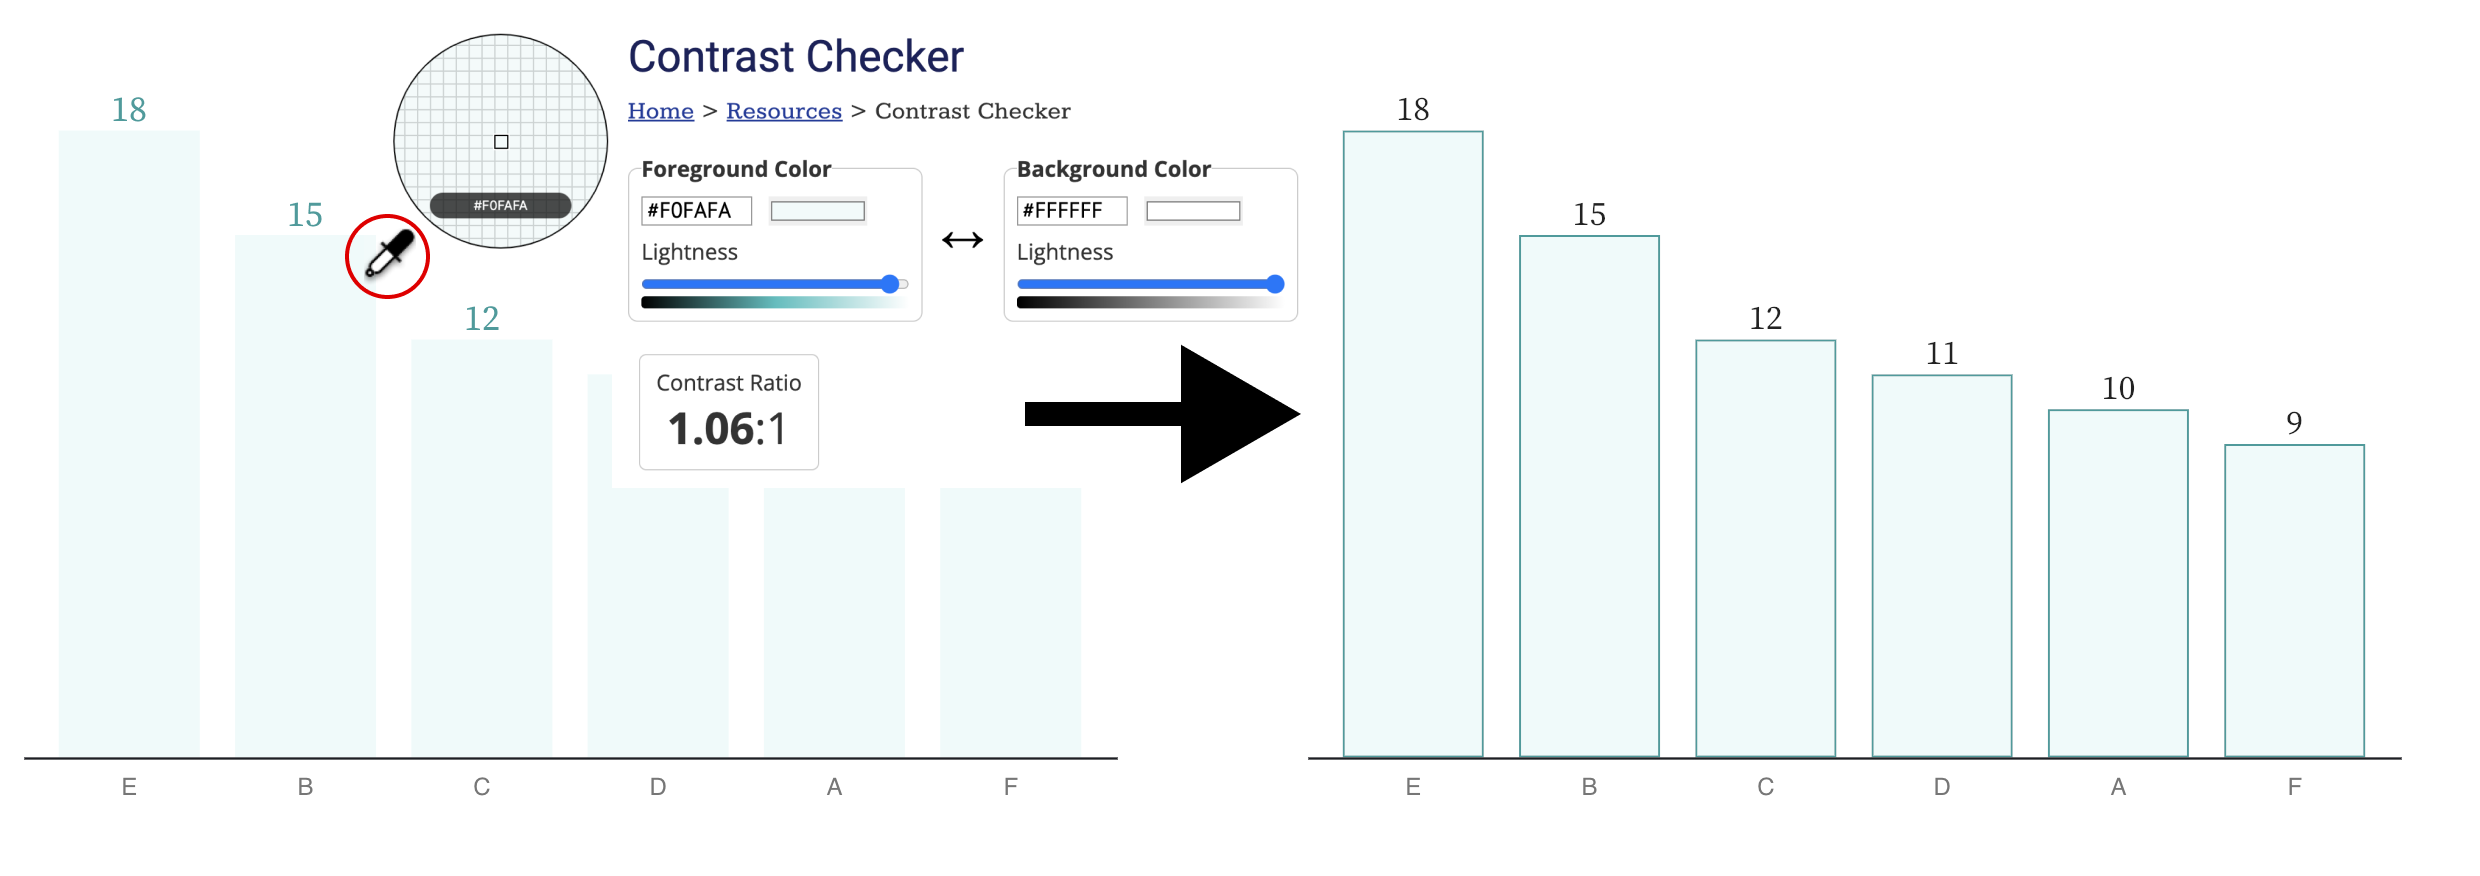
\includegraphics[width=\linewidth]{figures/figure 2.png}
    \caption{A low contrast chart (left) compared to a higher contrast version (right). A dropper tool is extracting the fill color of the bar and then a contrast ratio has been calculated. Note that the fill color is the same on both bars, but darker borders have been added to ensure the visualization passes contrast tests.}
    \label{fig:2}
\end{figure}

Checking for contrast is the most common critical failure; 87.5\% of tests (7 out of 8) from our user study involving this heuristic failed, which supports the WebAim Million Report’s findings (83.9\% of the top 1 million websites also fail contrast testing, more than any other WCAG criteria)~\cite{noauthor_webaim_nodate}. In order to evaluate contrast, often a combination of automatic (code-driven) and manual tooling is performed. When manually auditing, practitioners typically use a dropper and a contrast calculator (\autoref{fig:2}). Most auditors find this to be one of the easiest tasks to perform and accomplishes 3 different heuristics in Chartability: ensuring text/geometries have contrast, interactive states for elements have enough contrast change, and the keyboard focus indicator is easy to distinguish. 

Perceivable heuristics also include tests and tools for color vision deficiency and ensuring that color alone isn't used to communicate meaning (like the redundantly encoded textures in \autoref{fig:9}). And another common, critical failure from Perceivable is text size. No text should be smaller than 12px/9pt in size.

\begin{figure}
    \centering
    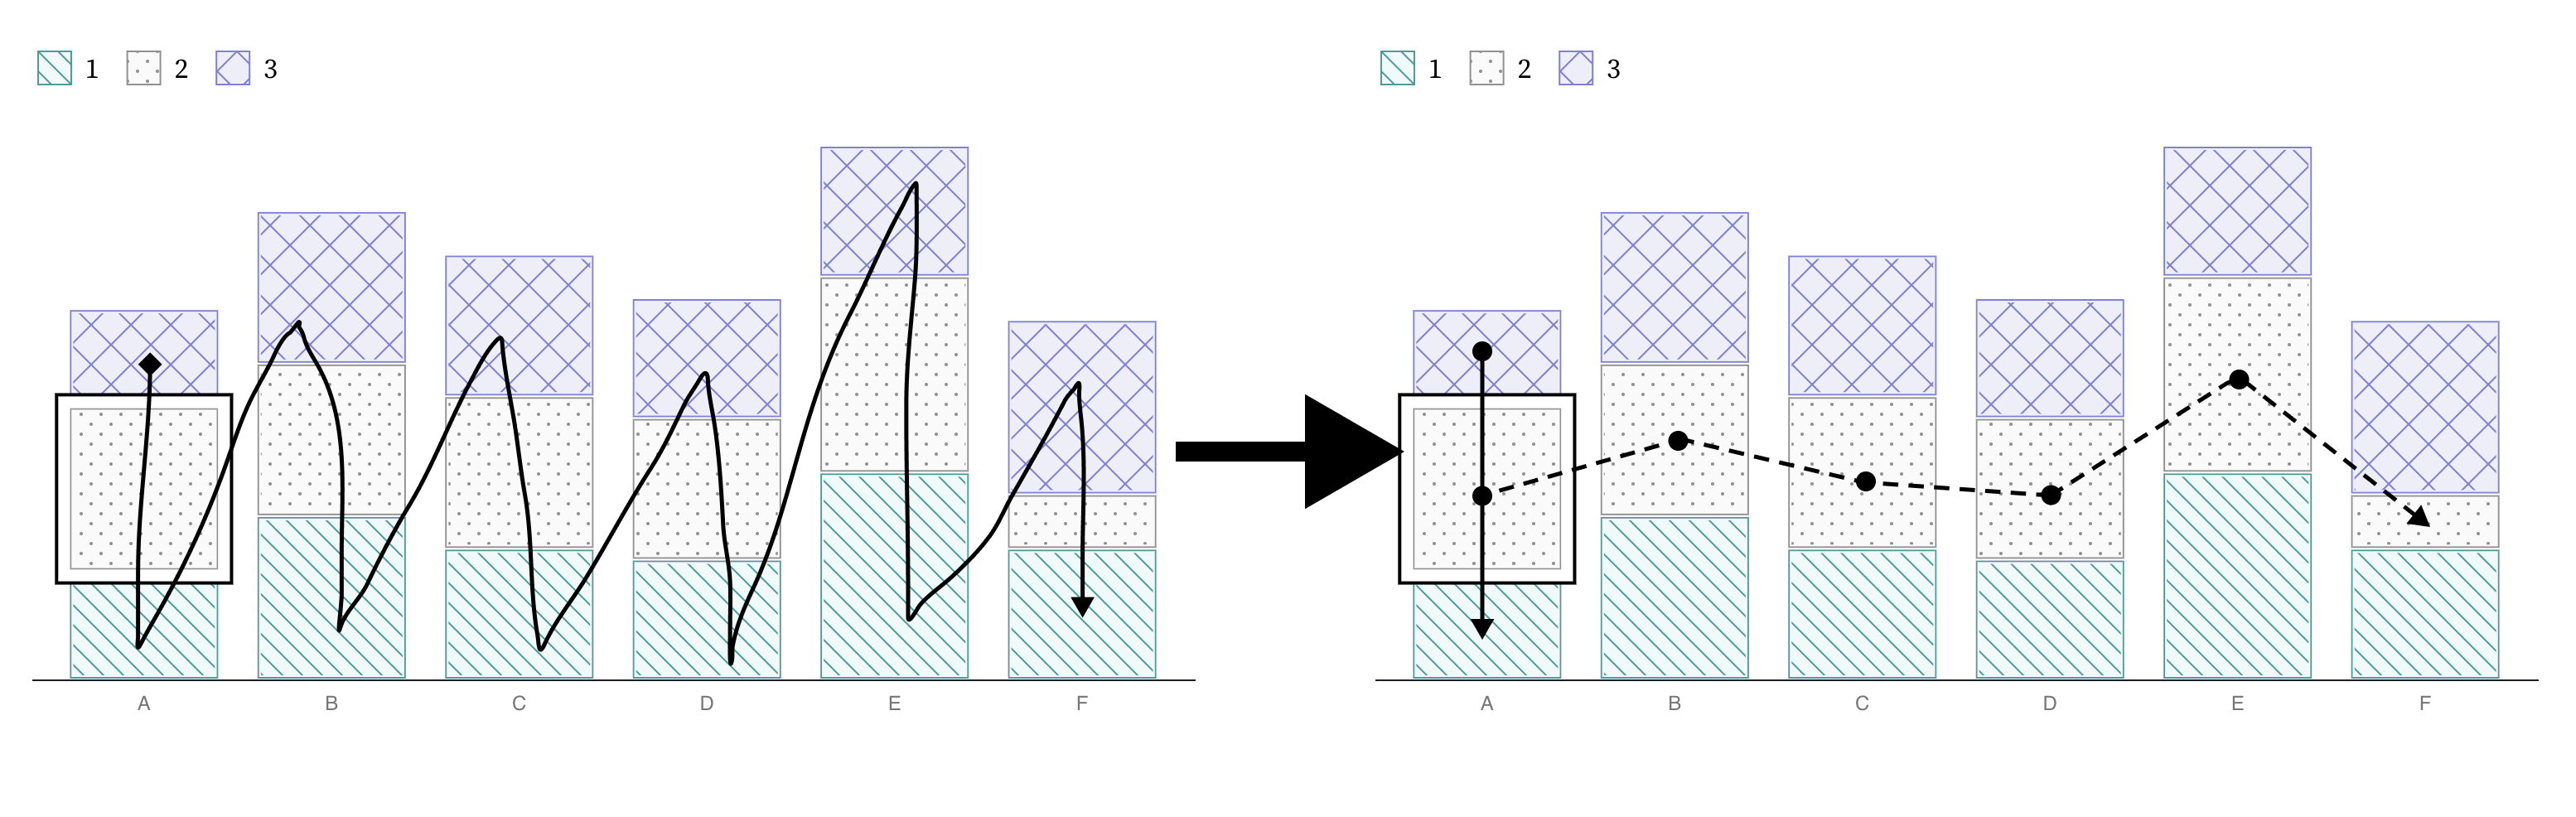
\includegraphics[width=\linewidth]{figures/figure 3.png}
    \caption{Keyboard navigation paths on a stacked bar chart. The left shows a serial navigation example, typically just a default of rendering order. The right shows both groups (the stack of bars) and categories (the color/texture shared among bars across stacks) as dimensions to explore laterally or vertically.}
    \label{fig:3}
\end{figure}

\subsection{Keyboard Probing (Operable, Assistive)}
The next practice that most auditors should become comfortable with is using a keyboard to navigate and operate any functionality that is provided. Most assistive technologies, from screen readers to a variety of input devices (like switches, joysticks, sip and puffs, etc) use the keyboard api (or keyboard interface) to navigate content. If a data interface contains interactive elements (\autoref{fig:3}, \autoref{fig:4}), those elements (or their functionality) must be able to be reached and controlled using a keyboard alone. Auditors should be critical of how much work is involved in keyboard navigation, especially (\autoref{fig:8}). All that is required to start is the auditor begins pressing the tab key to see if anything interactive comes into focus. Arrow keys, spacebar, enter, and escape may be used in some contexts. Generally, instructions or cues should always be provided.

\begin{figure}
    \centering
    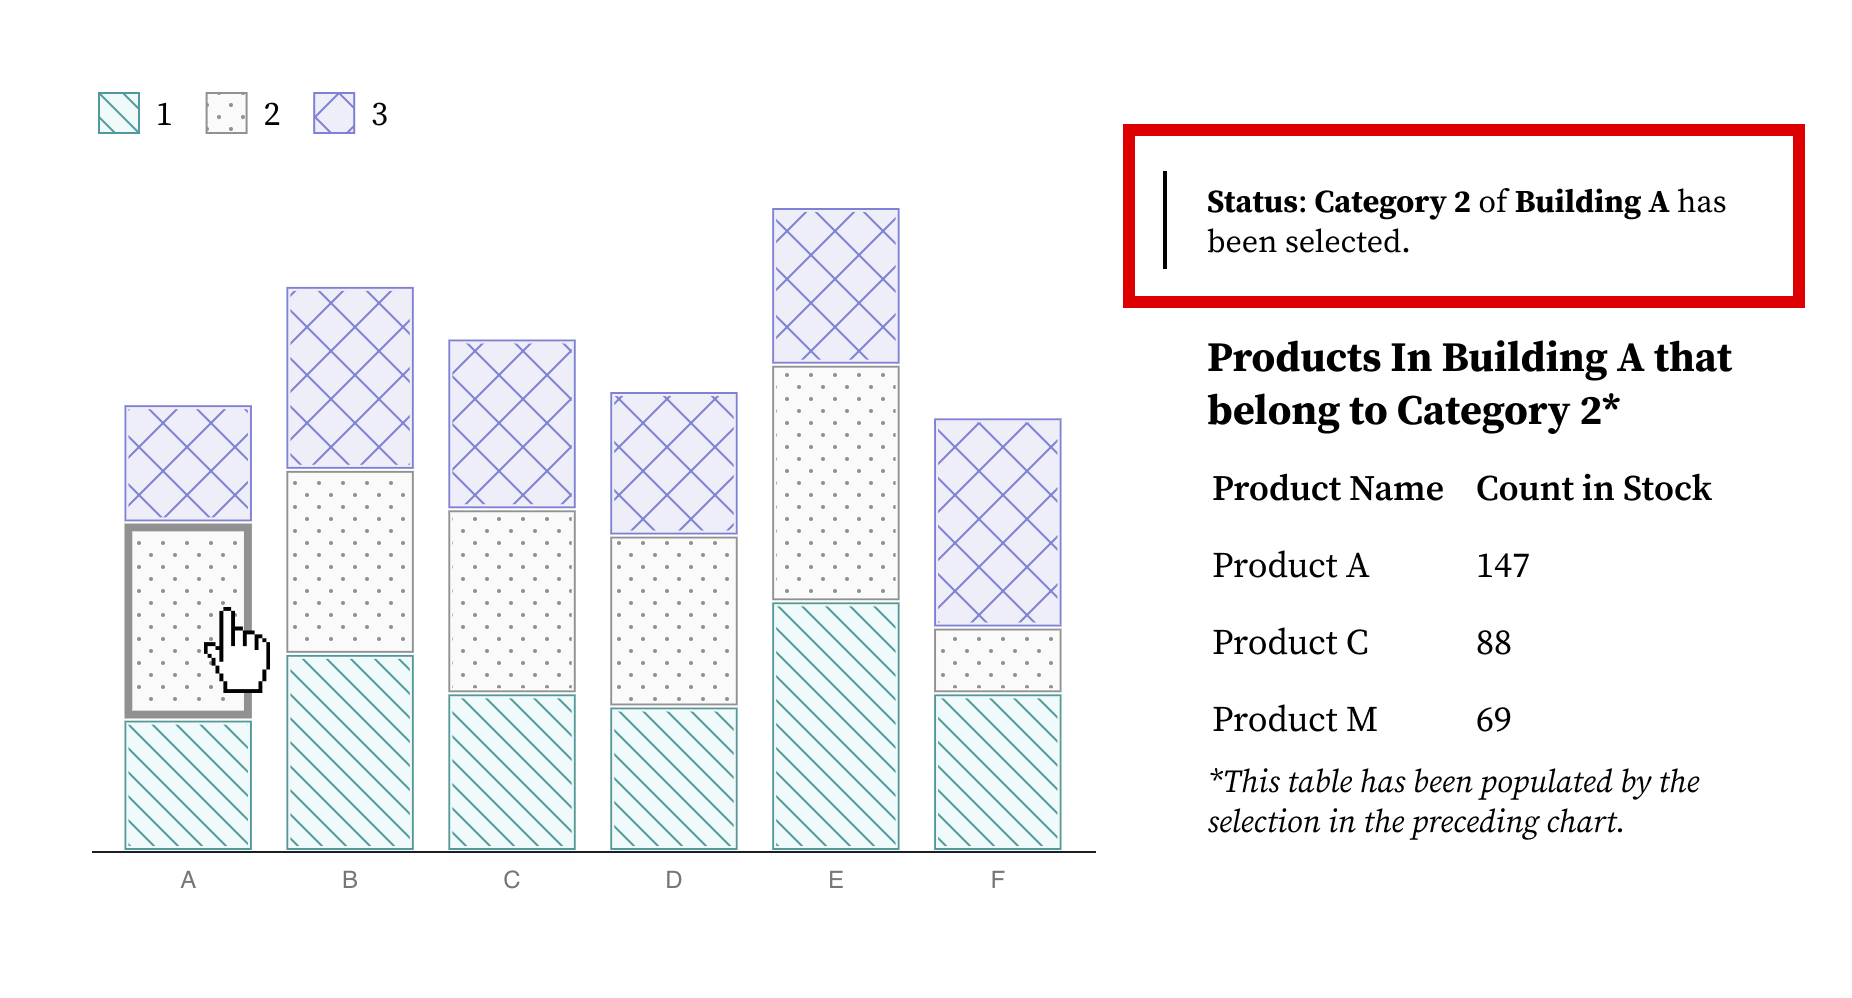
\includegraphics[width=\linewidth]{figures/figure 4.png}
    \caption{A mouse cursor is selecting a bar (left, shown with a thick indication border) in a stacked bar chart to filter a dataset (on the right). A system alert (red box) notifies the user of their interaction result. This selection capability must also be provided for the keyboard interface and the alert must be announced to screen readers.}
    \label{fig:4}
\end{figure}

Using a keyboard provides an opportunity to evaluate many different heuristics: checking for multiple inputs (\autoref{fig:4}), whether the data structure that is rendered is navigable according to its structure (\autoref{fig:3}), and whether keyboard navigability across all elements in a data interface is even necessary (\autoref{fig:8}).

\subsection{Screen Reader Inspecting (Perceivable, Operable, Robust, Assistive) }
Closely related to keyboard testing is testing with a screen reader. Some things may work with a screen reader that do not with a keyboard (and vice versa), so both must be evaluated.

\begin{figure}
    \centering
    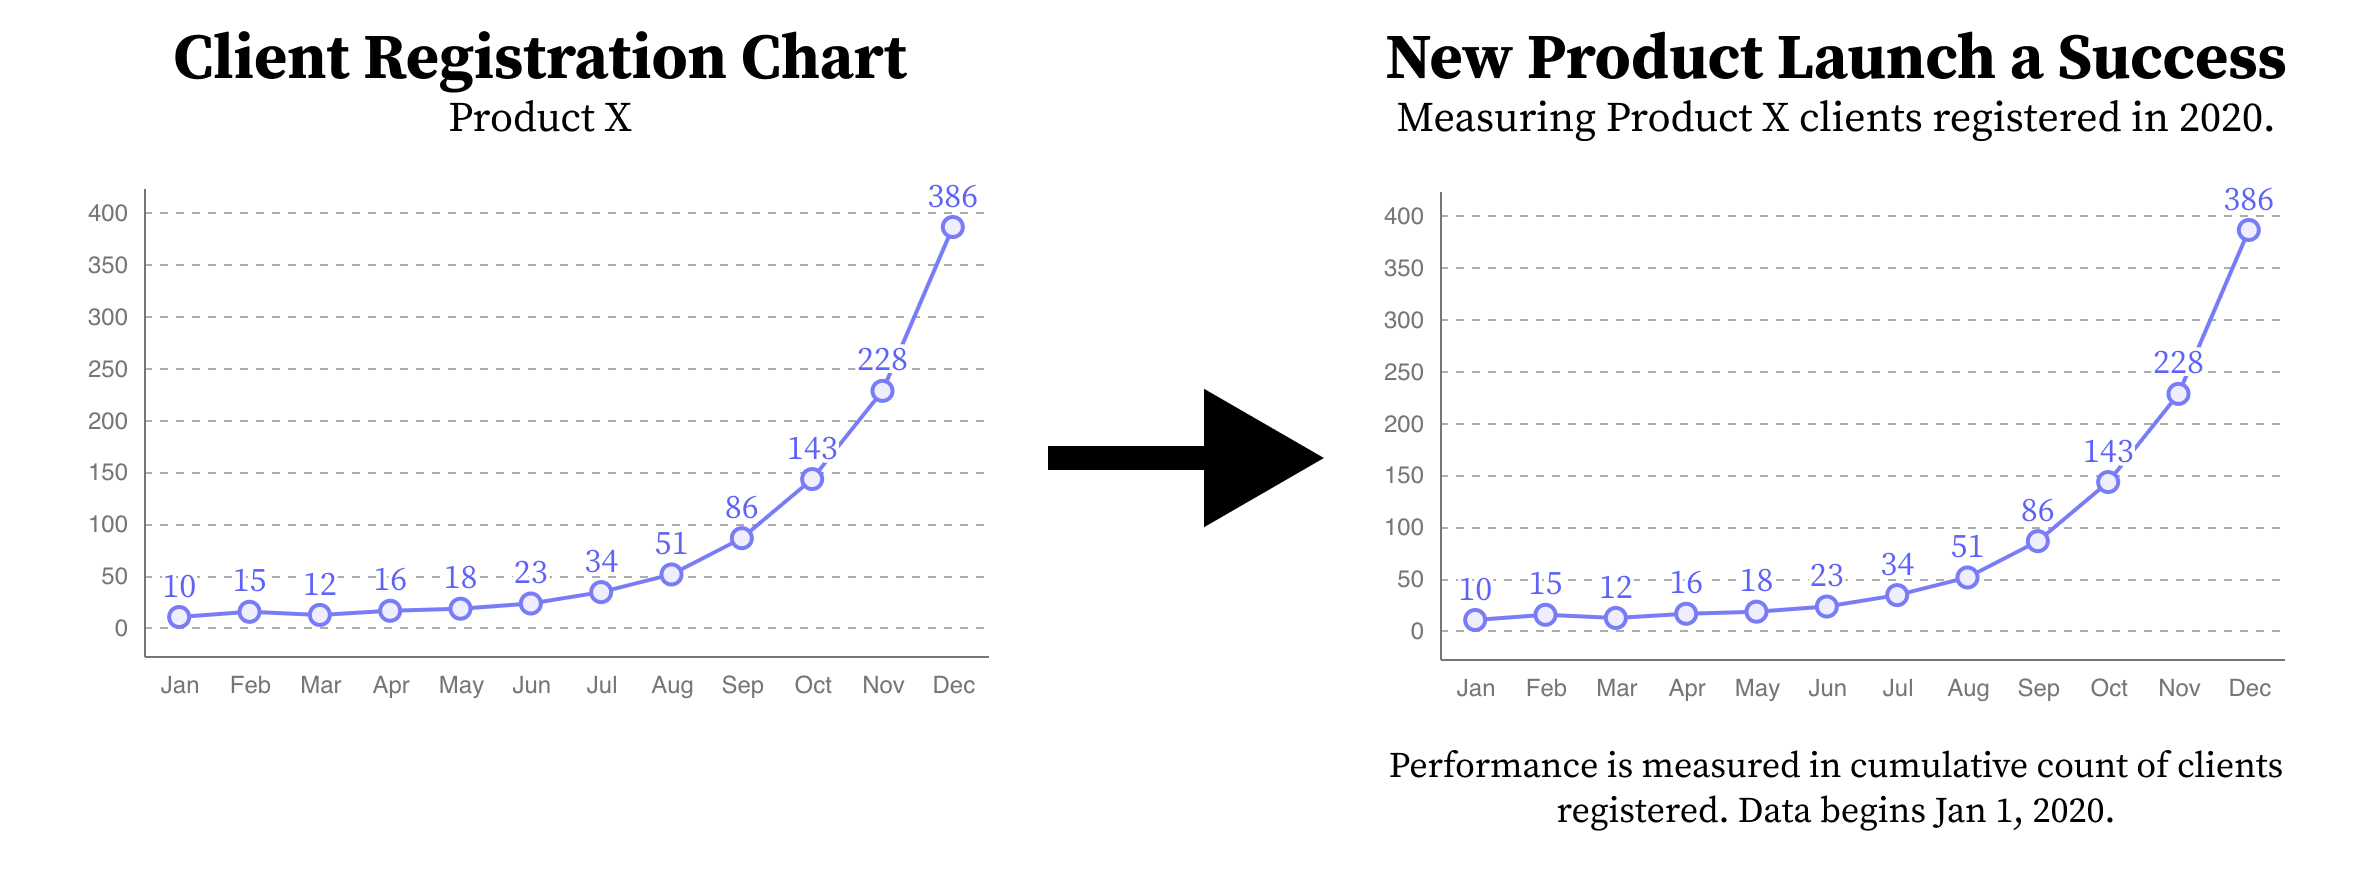
\includegraphics[width=\linewidth]{figures/figure 5.png}
    \caption{Charts must have a visually available textual explanation provided that summarizes the outcome. ``Client Registration Chart'' for ``Product X'' (left) is inaccessible while ``New Product Launch a Success'' (right) gives a clear takeaway.}
    \label{fig:5}
\end{figure}

Screen readers, unlike more basic keyboard input devices, read out content that is textual (including non-visual textual information like \emph{alternative text}). Using a screen reader to audit is generally the hardest skill to learn. Keeping this in mind, testing whether the meaningful text provided in a visual (such as in \autoref{fig:5}) is accessible with a screen reader is the easiest and most basic test that auditors should first perform.

\begin{figure}
    \centering
    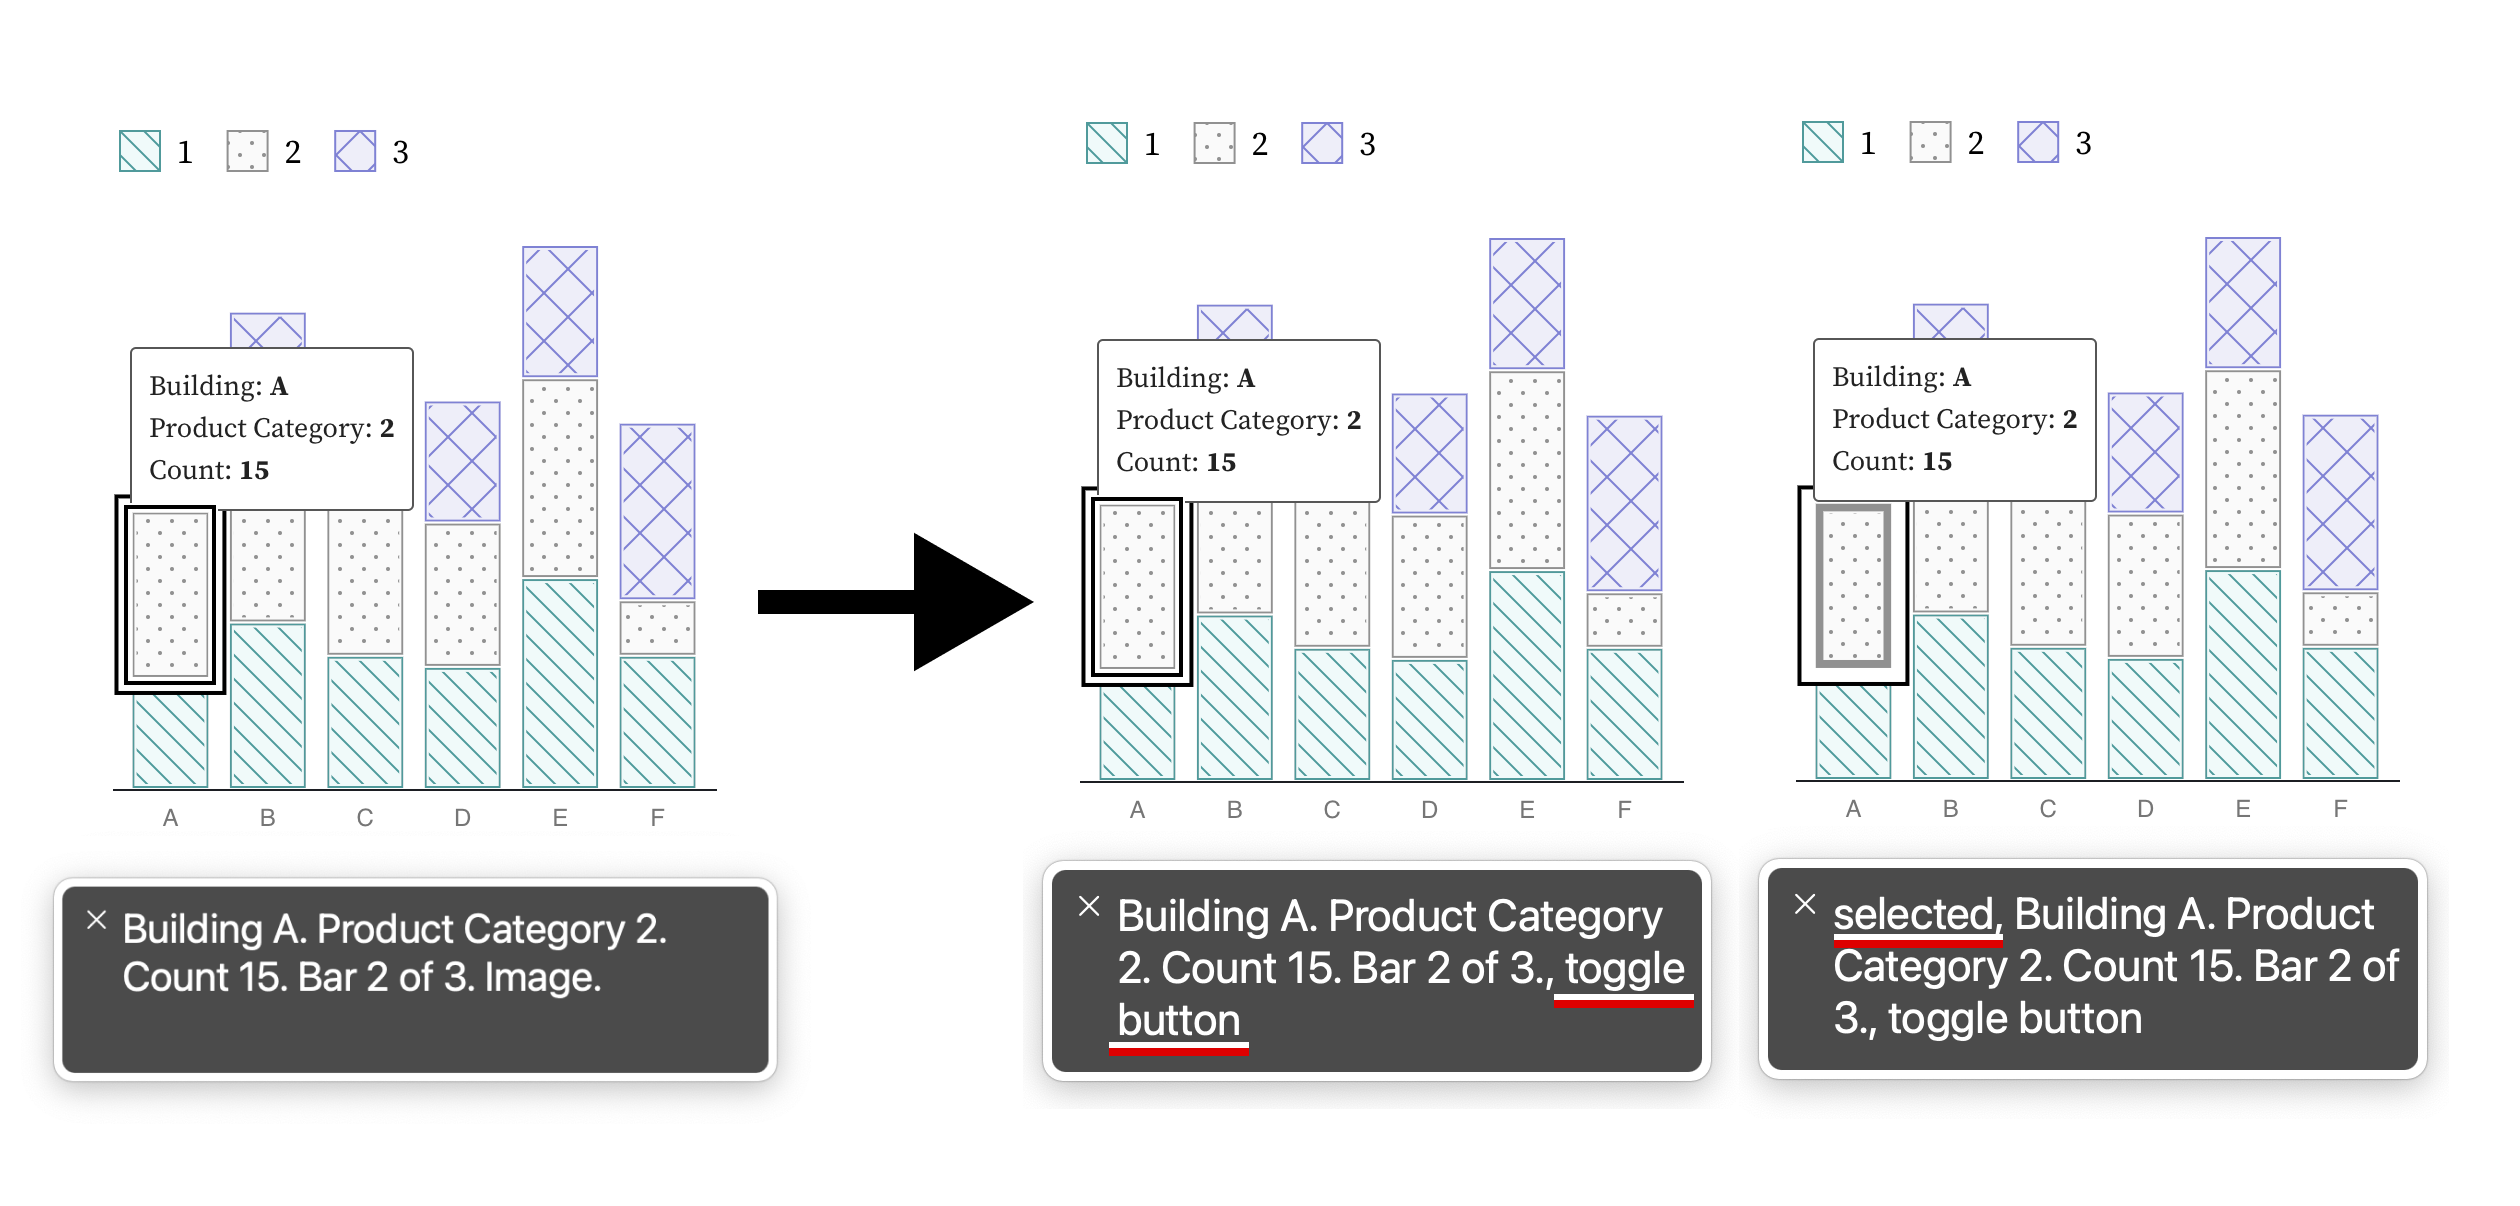
\includegraphics[width=\linewidth]{figures/figure 6.png}
    \caption{An interactive chart displaying only ``Image'' as semantic information with no feedback provided on selection. The robust semantics given to a screen reader, ``toggle button'' (middle) as well instant feedback, ``selected'' (right) are considered proper semantics for an interactive experience.}
    \label{fig:6}
\end{figure}

Next, all valuable information and functionality in a data experience should be tested whether it is available to a screen reader. This includes the individual variables about a mark as well as whether that mark is interactive (\autoref{fig:6}), whether status updates that reflect context change provide alerts (\autoref{fig:4}), and whether summary textual information is provided about the whole chart (\autoref{fig:5}) as well as statistically and visually important areas of that chart (\autoref{fig:8}). 

\begin{figure}
    \centering
    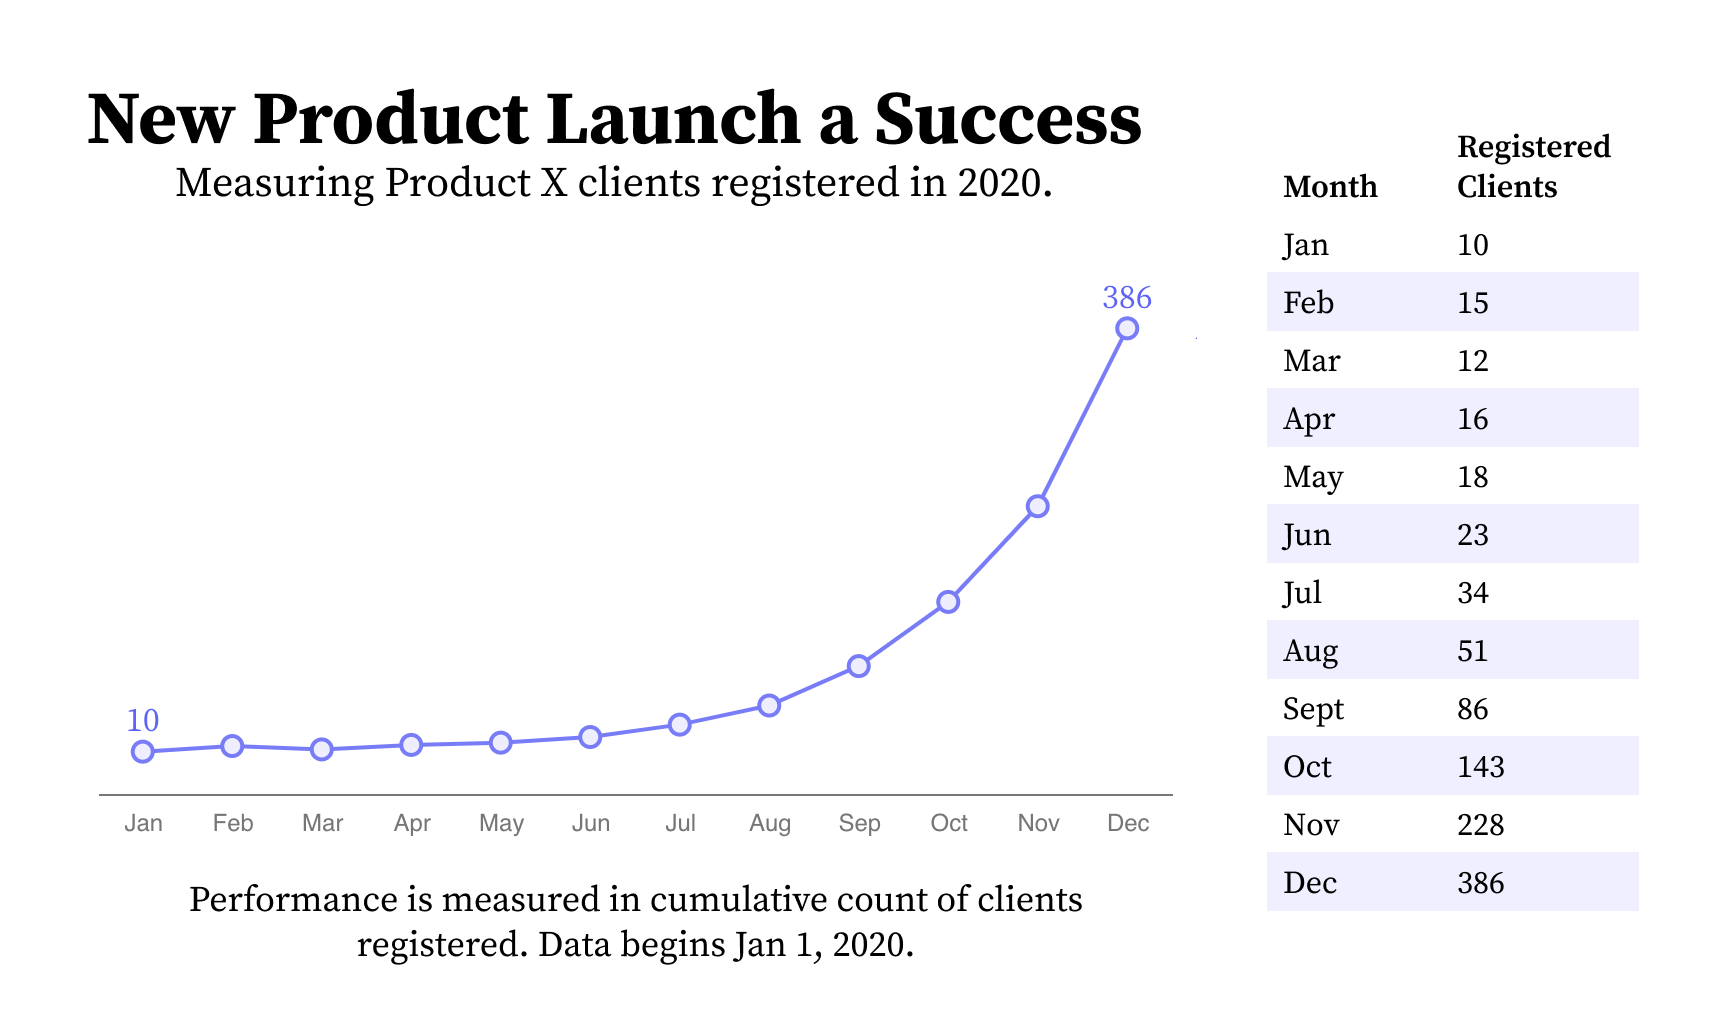
\includegraphics[width=\linewidth]{figures/figure 7.png}
    \caption{A line chart (left) with a single line and an accompanying data table (right). This line chart would not provide enough low-level information about each datapoint without the table provided. A table alone however would also be inaccessible. Providing both can satisfy conflicting accessibility needs for different audiences.}
    \label{fig:7}
\end{figure}

\subsection{Checking Cognitive Barriers (Understandable, Compromising)}
First, auditing for cognitive barriers generally involves checking the reading level and clarity of all available text using analytical tools. But Chartability also requires that all charts have basic text that provides a visually-available textual description and takeaway (\autoref{fig:5}). This alone is one of the most important things to check for. In complex cases where a chart has a visual feature with an assumedly obvious takeaway, checking for annotations or textual callouts is important to help avoid interpretive issues~\cite{xiong_curse_2020} (\autoref{fig:8}).

\begin{figure}
    \centering
    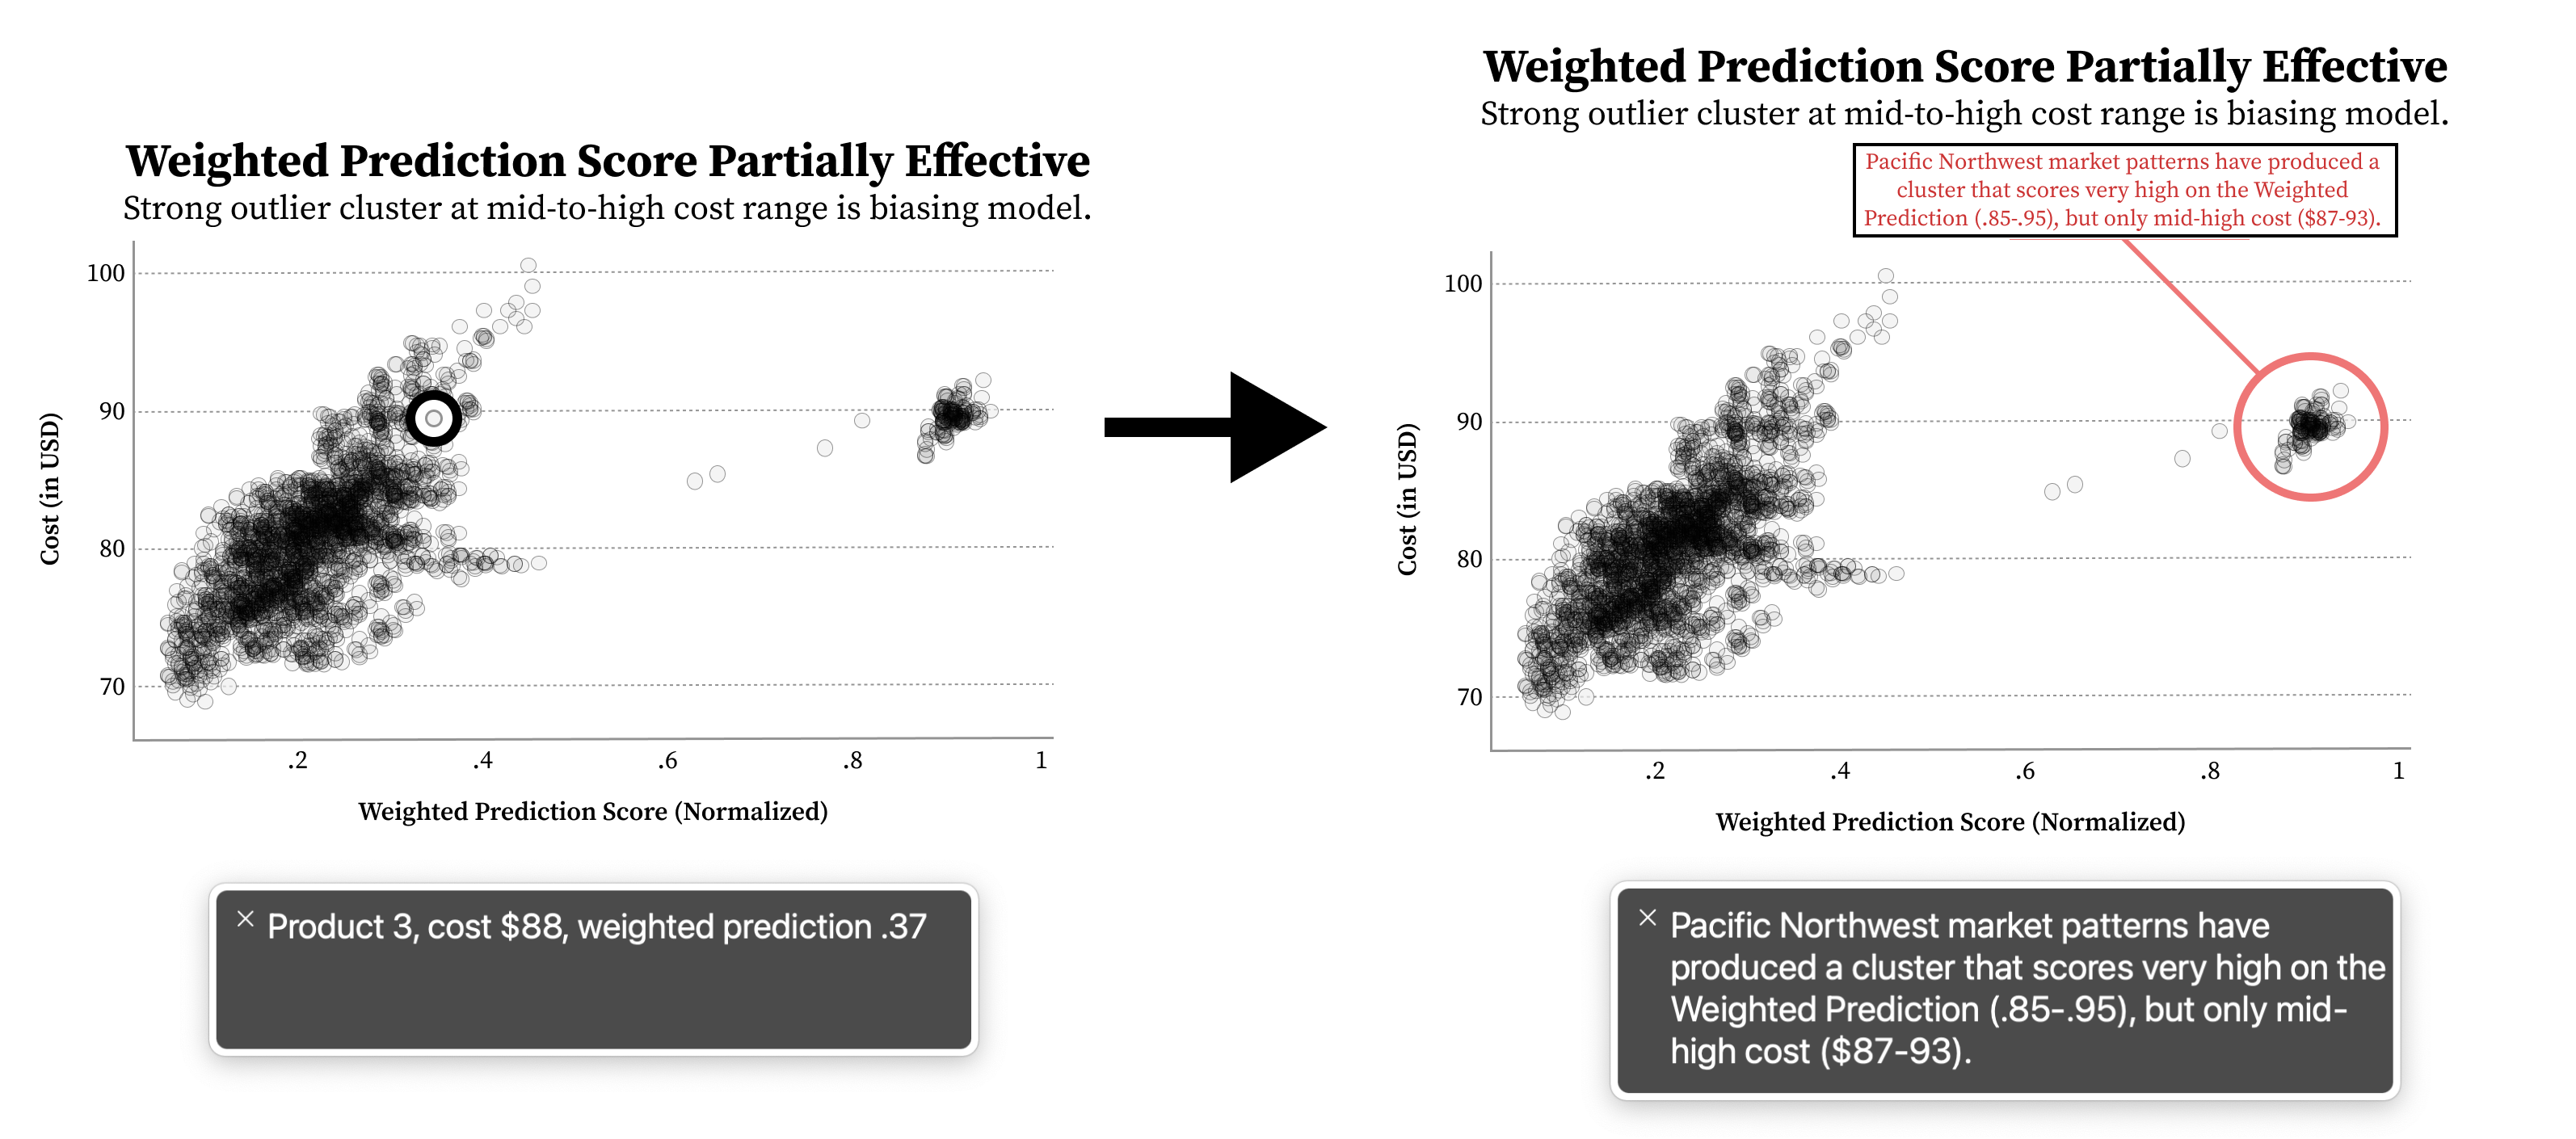
\includegraphics[width=\linewidth]{figures/figure 8.png}
    \caption{A scatterplot with many points, where a single point within the chart can be accessed by a screen reader (left). Navigating this data piece by piece is unnecessarily tedious, so an annotation callout is provided to help the reader focus on an outlier cluster (right). The callout is being accessed by a screen reader, which is displaying the annotation’s summary as well.}
    \label{fig:8}
\end{figure}

\subsection{Evaluating Context (Robust, Assistive, Flexible) }
The final series of checks an auditor should make involve thinking about the overall work in a design (as it intersects with other considerations) as well as the larger technical context where the user is situated.

Auditors should first try to change system settings (such as toggling high contrast modes) to see whether a data experience respects these settings (\autoref{fig:9}), run automatic semantic evaluations as well as manually check for appropriate meaning (\autoref{fig:6}), and check if dense or highly complex visuals have sonified, tactile, or textual summaries available (\autoref{fig:8}). Auditors should also check whether system updates provide clear feedback textually (\autoref{fig:4}) as well as checking if there are both high and low level representations of information available (\autoref{fig:7}).

\begin{figure}
    \centering
    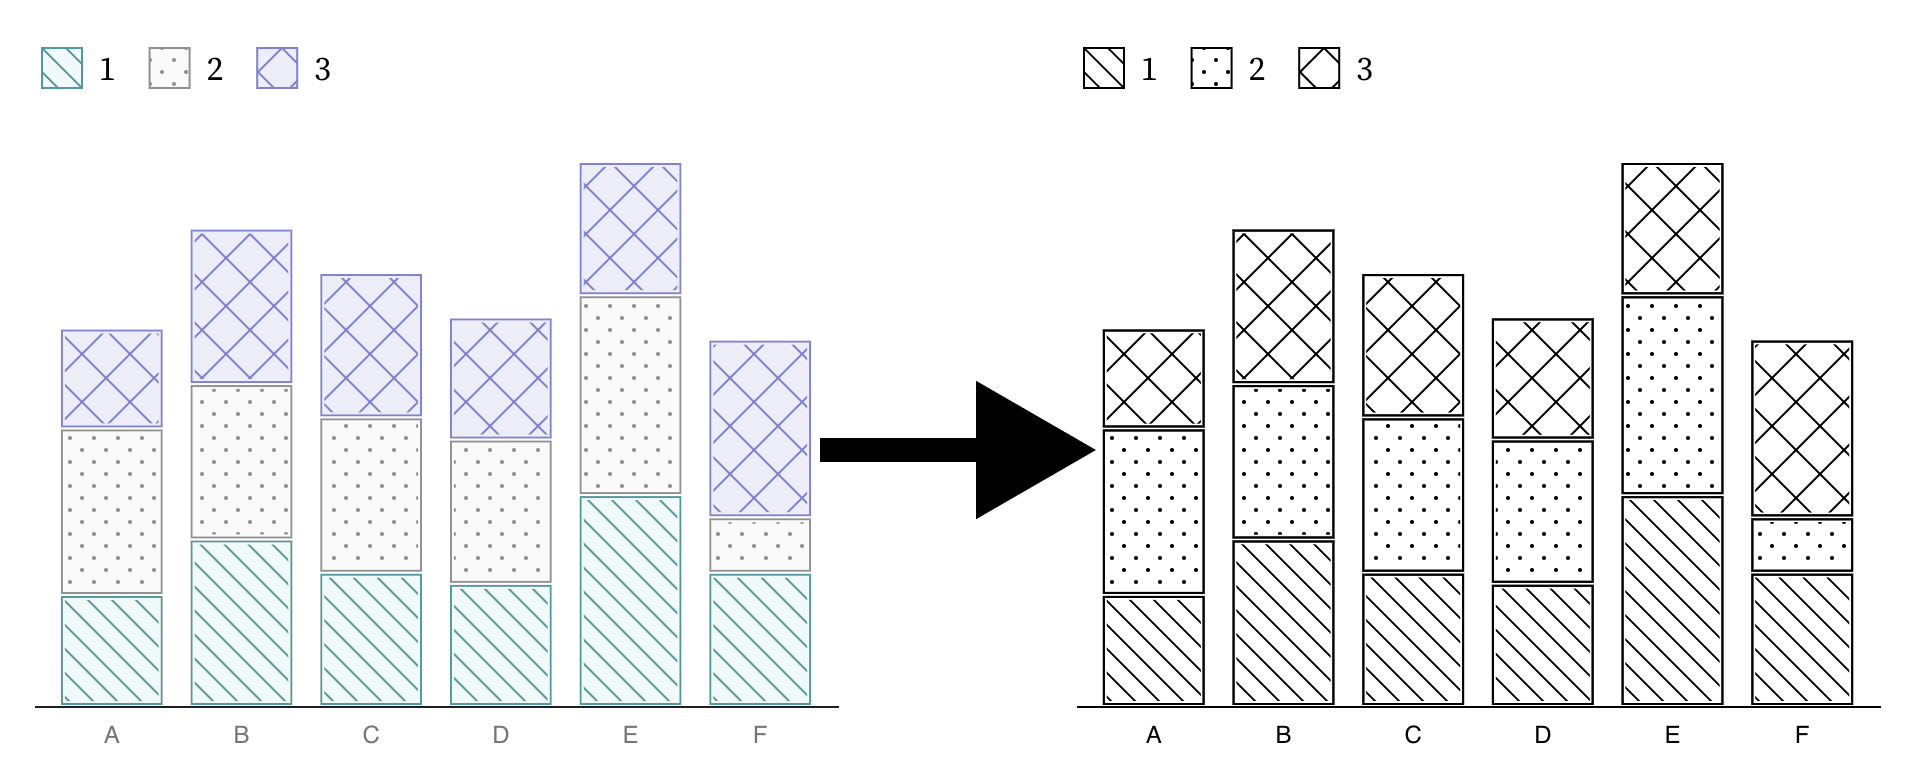
\includegraphics[width=\linewidth]{figures/figure 9.png}
    \caption{A bar chart with categories (left) shown not conforming to Windows High Contrast White Mode. High contrast mode on Windows requires limiting color palettes, using only black or white for most elements (shown on the right).}
    \label{fig:9}
\end{figure}

Auditors should be especially critical of static designs, such as those that either use textures by default or not (\autoref{fig:9}), which are a high risk of compromising and assistive failure.

\section{Validating Chartability}

Next, Elavsky explains the preliminary user evaluation: I validated whether data practitioners felt more confident and equipped to make their own work accessible with Chartability. Additionally, I also wanted to interview expert accessibility practitioners (including those with disabilities) with the same questions, to see if Chartability had anything to offer in helping them understand and evaluate data experiences better. 

My secondary goal was to present a tool that can be helpful even in the wild on real projects (with all the weird design and engineering quirks that come with that). I wanted Chartability to be usable on things built with a tool like Tableau and fully bespoke, hand-coded visualizations, like those made with JavaScript and D3. To this secondary aim, I intentionally solicited participants who were working on a variety of different projects, each of their own design. 

\subsection{Pre-Validations and Flipped Roles: Participants Question \emph{Me}}

I performed several early, light validations of my work before soliciting and involving participants formally. My early pre-validations \#2-4 (below) all focused on practitioners asking me questions and giving feedback. 

My 4 pre-validations happened during the process of making Chartability, as well as introducing short iterations back into the making process: 

\begin{enumerate}
    \item \textbf{Beta Testing}: I performed several beta tests of Chartability during the process of making. I audited using versions that only had POUR principles, tried versions of Chartability that focused only on standards, and also tried out different iterations of the heuristics as I was forming them. This testing was important to perform early in the process because it helped me test the limits of various possible directions for this tool (standards-only, against standards, building off of standards, etc).
    \item \textbf{Early Advice}: After the first full pass of making Chartability was complete, I sent Chartability via email to 4 accessibility experts and 6 interested people with disabilities familiar with auditing in order to solicit open feedback. 
    \item \textbf{Professional Workshop}: I held a half-day professional workshop via zoom on auditing visualizations for accessibility and presented Chartability’s heuristics to this select audience of 50 participants. I demonstrated how to audit and then had a chance for feedback and questions.
    \item \textbf{Deep Feedback Session}: I presented Chartability to 14 experts on data visualization and accessibility, 5 of which are people with disabilities. I presented in two separate sessions through 2-hour video calls on zoom (roughly one hour was demonstration and one hour was discussion). 
\end{enumerate}

\subsection{Discovering ``Critical'' Heuristics}
\label{sec:critical heuristics}
These pre-validations helped me combine and divide some of the heuristics, adjust the language and phrasing, and label 10 specific tests as ``Critical,'' which can be seen in \autoref{tab:table}. These critical tests were ones that community members stressed as an important priority for one or more of the following reasons:
\begin{itemize}
    \item They are prohibitively expensive to fix late.
    \item The barriers they produce are too significant to ignore.
    \item They are among the most common type of accessibility failure.
    \item They affect many parts of a data experience.
\end{itemize}

All Critical heuristics are based on standards or research.

\subsection{Selecting Participants and Projects}
I was a practitioner and representing myself as a volunteer when I reached out to participants. At this stage in the project, I was still not affiliated with a research institution and was not interested in producing publishable knowledge. I intended to test Chartability in the wild and validate whether it achieved its aims. My priority was to collaborate with folks working on difficult problems or those who had a rare intersection of expertise between accessibility standards and interactive data experiences. To this end, I was highly permissive with potential collaborators in order to maximize the expertise of participants and breadth of environments for testing Chartability. 

However, part of being permissive with participants meant that I was willing to collaborate on projects that I cannot share in a research publication and many of my participants must remain anonymous (including interview results that contain sensitive information about intellectual property). Given that auditing is a field of work about identifying failures, there was both a high demand for participation in the evaluation of Chartability in tension with a low motivation to make these failures known in a public venue.

A summary of our selection process:
\begin{itemize}
    \item \textbf{Solicitation}: I reached out via email to 24 individuals in my network to participate in helping to evaluate Chartability. I mentioned that I wanted Chartability to be applied to a current project of theirs and was interested in performing some interviews about their experience before and after using Chartability. I mentioned up front that working with me would be uncompensated and potentially take multiple hours of their time (even multiple sessions) over zoom meetings.
    \item \textbf{Response}: 16 individuals were interested and shared their project details (2 would require an NDA to be signed). 
    \item \textbf{Selection}: I selected 8, based either on the expertise of the individuals, on the robustness of their project, and/or on the opportunity to get feedback about Chartability in team environments (which I didn't anticipate, but 3 of the 8 represented team efforts).
    \item \textbf{Resulting Group}: I worked with 19 total participants across 8 environment spaces.
    \item \textbf{Publishable Group}: Due to intellectual property concerns, I can publish interview results from 6 participants and discuss the details of 4 audit environments.
\end{itemize}

\textbf{Chris DeMartini}: a multi-year Tableau Zen Master and recognized expert visualization practitioner. His dashboard of a coin flipping probability game dataset that he produced with his daughter was the subject of his audit~\cite{noauthor_we_nodate}. His audit only included criteria labelled Critical in Chartability (which involves only 10 tests instead of the full 45) and his dashboard failed 7 of them. A full audit was later conducted on Chris’s behalf. His full audit had a total 26 failures, 11 of which were considered non-applicable.\footnote{``Non-applicable:'' any test in the auditing process that that does not contain content relevant to the test, such as ``Scrolling experiences cannot be adjusted or opted out of'' for a visualization that does not a scrolling input control\label{fnlabel}}

\textbf{Amber Thomas}: a data storyteller and technologist credited on 30 of The Pudding's visual essays. Amber has had a growing interest in accessibility challenges related to her line of work designing and developing state of the art, bespoke visual essays. Her article The Naked Truth was still in the early design and development stages when it was fully audited~\cite{noauthor_naked_nodate}. It failed 22 out of 45 tests, including 6 out of 10 criteria considered Critical. 6 tests were considered non-applicable.\footref{fnlabel}

\textbf{Sam} (self-selected pseudonym): a recognized design practitioner in the visualization community who lives with disability. They were collaborating on an interactive data project that would be specifically made to be used by international participants with a broad spectrum of disabilities. Their interactive infographic failed 21 out of 45 tests, 5 of which were considered Critical. 10 tests were considered non-applicable.\footref{fnlabel}

\textbf{Øystein Moseng}: Core Developer and Head of Accessibility of Highcharts. Øystein was interested in taking one of Highchart’s demo charts not specifically developed with accessibility features in mind~\cite{noauthor_fixed_nodate} and testing it against a full Chartability audit to see how it held up. The demo failed 13 out of 45 tests, 3 of which were Critical. 10 tests were considered non-applicable.\footref{fnlabel}

\textbf{Jennifer Zhang}: a senior accessibility program manager at Microsoft with expertise working on enterprise data products.

\textbf{Ryan Shugart}: a blind, screen reader user and disability subject matter expert at Microsoft who has a strong expertise in collaborative accessibility for interactive data systems. 

Both Shugart and Zhang were interested in applying Chartability internally and testing its effectiveness and potential with various projects. Their application and use of Chartability (including audits) are not available for publication, but their valuable interviews and evaluations are included with permission.

% *``Non-applicable:'' any test in the auditing process that that does not contain content relevant to the test, such as ``Scrolling experiences cannot be adjusted or opted out of'' for a visualization that does not a scrolling input control.

\section{Study Results}

I asked the 6 participants a series of qualitative and Likert-scale evaluation questions:

\begin{enumerate}
  \item Have you ever performed an audit of a data experience before?
  \item What stage of production is your project in? Analysis, design, prototyping, development, maintenance?
  \item How confident are you in your ability to perform an audit of a data experience for accessibility issues? (1-5, 1 being not confident at all, 5 being fully confident.)
  \item How difficult do you perceive auditing a data experience for accessibility issues is? (1-5, 1 being trivial, 5 being very difficult.)
  \item (After using Chartability) How confident are you in your ability to perform an audit of a data experience for accessibility issues? (1-5, 1 being not confident at all, 5 being fully confident.)
  \item (After using Chartability) How difficult do you perceive auditing a data experience for accessibility issues is? (1-5, 1 being trivial, 5 being very difficult.)
  \item (After using Chartability) Do you intend to continue using Chartability?
\end{enumerate}

Each of these questions had an open-ended question attached, ``Is there anything else you would like to add?'' Every participant provided additional input on questions 3 through 7. 

None of the 3 participants who only consider themselves expert data practitioners had performed an audit before. All 3 of them reported that they believed auditing to be easier and that they are more confident in their ability to evaluate the accessibility of data experiences after using Chartability. 

Of the 3 accessibility experts (all of whom have performed audits of data experiences before), their opinions on these measurements were unchanged after using Chartability. All 6 participants noted that they plan to use Chartability in their own work and would recommend it to their peers. 

Below we overview some of the key insights Elavsky received from the open ended responses.

\subsection{Real Access has more Considerations than Colorblindness}
Among the data practitioners, DeMartini wrote after his audit, ``I have read a lot about color blindness and could provide meaningful feedback to visualization developers on that topic, but I have come to realize that accessibility is so much more than this and I basically didn’t really know where to start when it came to the true scope of accessibility.'' He ended his qualitative feedback with, ``I think this could be a great tool for the masses and really look forward to the impact it can possibly have on the (inaccessible) data visualizations which are being created in huge numbers these days.''

\subsection{Audits are Slow, but Help me Focus}
Amber Thomas wrote, ``It still takes a while to do a complete audit, but it's not hard! For someone new to the space, all the possible options that can be used to make visualizations more accessible can be overwhelming. [Chartability] helped me to focus.'' She finished her feedback with, ``There aren't really guidelines (at least to my knowledge) that exist to help data visualization creators to ensure their work is accessible… [Chartability] helps to direct users to the most common accessibility problems with straightforward questions. It really helps to narrow the focus and prioritize efforts.'' 

\subsection{Chartability Helps me Remember and Stay Consistent}
Among the accessibility experts, Zhang wrote, ``While I am skilled, depending on the day I might not remember everything I need to look at. I am more confident in consistency between different auditing sessions. For experts it’s a good reminder framework.'' Moseng of Highcharts noted, ``[Chartability] did a very good job of highlighting concerns that are often ignored or forgotten when auditing and designing/developing.'' Shugart of Microsoft added along those lines, ``I feel [Chartability] arranges a good set of questions in a user’s mind and makes it easier for them to determine if a visualization is accessible.''

\subsection{Access is an Experience, not just Compliance}
Zhang offered insight into the design intention of Chartability, ``[it is] clearly going for above compliance and focusing on a good experience.'' Sam expressed their need to make an excellent accessibility experience, ``I am not just worried about compliance, but I want to make something really good. Nothing seems to help you go beyond? This is better than WCAG, I can already tell.''

\subsection{Everyone wants More Evaluation Resources and Tools}
For constructive feedback, all the data experts noted that they wanted more resources and materials related to learning the skills needed to conduct an audit. Shugart and Moseng both noted that they hope for more tooling and (in some cases) automated tests that can take the burden off the auditor and streamline the design and development process (much like Axe-core~\cite{noauthor_axe-core_2021}). They both also agreed that automation and tooling would help novice practitioners perform this work faster and with more confidence. 2 of the 3 mentioned wanting more examples of failures as well as accessible data experiences. Sam wrote that they felt Chartability was overwhelming at first, but after focusing on just the Critical items, the rest of the framework ``became easier.''

\subsection{Experts: ``Novices will Struggle.'' Novices: ``This was so helpful''}
The accessibility experts all unanimously agreed that Chartability is helpful to their own work, but they are unsure how accessibility novices would do. They all believe that more training and resources are needed to help people who are new, with one noting that Chartability could even be ``overwhelming'' to someone who has not been exposed to accessibility work before. All of the novices remarked that Chartability was ``so helpful,'' ``made this work so much clearer than before,'' and ``made a lot of hard problems not as hard.''

\subsection{What about Auditors with Disabilities?}
Shugart’s feedback was critical when discussing continuing to use Chartability, ``I still feel as a screen reader user, the audit itself would have some unique challenges because I’d be missing a lot and would have problems determining things such as color.'' He continued, ``Auditing anything accessibility-wise as a screen reader user poses challenges because you don’t always know what you’re missing. In many cases there are workarounds to this but datavis is one area where this is really hard to do now.'' 

\section{Extended Results}
Following calls to ensure accessibility work has practical benefits that exceed publications~\cite{hurst_making_2013}, in April, 2021 Elavsky made Chartability openly available on Github. As new research and practices emerge and more community members get involved, Chartability will become an evolving artifact of consensus similar to existing standards bodies~\cite{noauthor_w3c_nodate}.

Projects like Turkopticon benefited from the discussion about how a community actually used their tool~\cite{irani_turkopticon_13}. In the same vein, we are happy to report some valuable findings from within this last year that we think demonstrate (in a pragmatic way) that Chartability has some merit: 
\begin{itemize}
    \item \textbf{It is living and growing}: Chartability has received enough community feedback that it is now on Version 2, with more tests and background resources provided.
    \item \textbf{People are talking about it}: Chartability has been featured in 14 workshops, talks, and podcasts and at least 2 university courses.
    \item \textbf{People are using it}: Chartability has contributed to projects at Microsoft, Highcharts, Project Jupyter, Fizz Studio, FiveThirtyEight, Vega-Lite, UCLA, the City of San Francisco, the Missouri School of Journalism, a fortune 50 company, two Fortune 500 companies, and community groups (like MiR).
    \item \textbf{It has breadth}: Chartability has evaluated static and interactive data experiences made with Microsoft's Excel and PowerBI, Tableau, JavaScript (D3, Vega-Lite, Highcharts, Visa Chart Components), Python (Altair, Bokeh, and matplotlib), R (ggplot2), as well as design sketches and low/medium-fidelity artifacts (Illustrator, Figma, Sketch).
\end{itemize}

When considering the analysis by Hurst and Kane about high abandonment rates in assistive technology,~\cite{hurst_making_2013} we wanted to make sure that we created an artifact (assistive technology or otherwise) that would at least survive its first year of use in the real world. 

The greater community feedback as well as new research before and after open-sourcing Chartability has also led to 5 new heuristics being added since our test users performed audits and gave evaluations. The current version of Chartability (v2) has a total of 50 heuristics. 

It is important to note that the work of Chartability did not begin and does not conclude with the publication of this manuscript. We want Chartability to become a living, community-driven effort that will adapt and grow as more resources, tools, and research become available.

\section{Discussion}
From our presentation of Chartability and a preliminary user evaluation with data visualization and accessibility practitioners, we learned that Chartability reduced the perception that working on accessibility is difficult and increased the confidence of those new to this work. Chartability shows promise as a useful framework for expert accessibility practitioners because it serves to produce consistency in contexts like the evaluation of dashboards, data science workflows, and other complex, data-driven interfaces. 

While our practitioners with novice accessibility experience were initially concerned about doing the audit correctly, most of their audit results were reasonably comparable with that of the authors (although their time to complete was much longer). 

We agree with experts that beyond Chartability, more resources are needed which provide examples of both inaccessible and accessible data visualizations as well as how to perform some of the more difficult parts of the auditing process (such as evaluating with a screen reader). We hope that keeping Chartability on GitHub will inspire future improvements to address this gap in examples, and will address future limitations, as we discover them. 

Chartability is a valuable tool for auditing. But we also hope that it can inspire researchers to:
\begin{enumerate}
    \item Examine which heuristics (in our supplemental materials) could use more research attention, particularly those labelled ``community practice.''
    \item Define constraints or requirements on novel projects, ensuring that new explorations still respects established standards, mitigating ethical risks.
    \item Explore the intersections of disability in ways yet unaddressed in standards, such as the strong overlaps between understandability and operability (like keyboard navigation patterns across a data structure) or conflicts in understandability and flexibility (how some users need redundant encodings on charts while others find this overwhelming).
    \item Consider access barriers in data experiences beyond those related to visual perception.
    \item Engage the relationship between labor and access in computing, such as developing more measurements that demonstrate the imbalance of time and effort expected of users with disabilities (even in systems considered to provide ``equal'' access) and ways to evaluate who is contributing to accessibility efforts in a project (core team members, contractors, or volunteers).
\end{enumerate}

We also want to caution researchers who are considering developing heuristics or auditing tools for use in practitioner environments to consider the tradeoffs between evaluation in rich, authentic professional settings and concerns such as intellectual property and corporate branding. We were able to apply our work in rich and collaborative practitioner settings because we were permissive with our potential participants. However, much of this work exists behind closed doors, similar to the downsides of industry research settings. More work may need to be done in order to encourage rich, cross-industry research projects, such as helping to anonymize the content of intellectual property and not just participants, while retaining data and findings. 

\section{Conclusion}

The demand for accessible data experiences is long overdue. The Web Accessibility Initiative’s (WAI) Web Content Accessibility Guidelines (WCAG) are over 22 years old and yet little work has been done to synthesize this large body of existing accessibility standards with research and inclusive design principles relevant to the fields of data communication, data science, data analysis, and visualization. Chartability begins to address unique accessibility best practice gaps in these domains with specific heuristics. This synthesis is meant to empower researchers, analysts, designers, developers, editors, and accessibility specialists with a framework to audit the accessibility of data experiences, interfaces, and systems to produce more inclusive environments for users with disabilities. The goal of Chartability is to make this work easier in order to encourage practitioners to regard current practices and resources, some of which have existed for decades. 

In addition, Chartability opens the door to more work that remains to be explored in this space. Additional research is needed into many of the topic areas within Chartability’s heuristic principles (POUR+CAF) as well as resources, examples, and tools provided for practitioners to perform this work more confidently and efficiently. 

The changing landscape of visualization techniques and alternative interfaces (such as sonification and dynamic tactile graphics) may increase the demands for accessibility considerations in this space. The growing technological divide will become an even greater human rights issue as time moves on and we believe that tools like Chartability are necessary for the community of data practitioners to ensure they are including people with disabilities.

\section*{Acknowledgements}
First we want to thank our reviewers. This paper would not have found its core contribution without your help. 

We especially want to thank all the community members who helped contribute to improving Chartability during the making process as well as after we released (in no particular order): Liz Hare, Silvia Canelón, Léonie Watson, Emily Kund, Sarah Fossheim, Ted Gies, Larene Le Gassick, Melanie Mazanec, Amanda Makulec, Amy Cesal, and anonymous friends. We also want to thank all of our industry partners who are currently using Chartability.

And lastly, special thanks to Doug Schepers of Fizz Studio for sponsoring Chartability and for your gracious encouragement, support, and feedback. 

% bibtex

\bibliographystyle{eg-alpha-doi}  
\bibliography{bibliography}        

% biblatex with biber
% \printbibliography                

\end{document}
